% Mingyu Xia (夏明宇, Westlake ID: 20251202247) Homework #i & #j
\documentclass[11pt]{book}

\usepackage[cache = false]{minted}
\usepackage{float}
\usepackage[natbib, style = phys, biblabel = brackets, sorting = none]{biblatex}
\addbibresource{reference-phx.bib}
\addbibresource{reference-math.bib}

\makeatletter
\def\input@path{{../}}
\makeatother
\usepackage{preamble}


\coverset{
  title   = Advanced Quantum Mechanics,
  author  = \ttfamily \textsc{Mingyu Xia},
  afill   = PhD @Westlake University,
  date    = November 2025,
  extinfo = {\includegraphics[width = .1\paperwidth]{myhsia_seal}},
  head    = universe.pdf,
  clogo   = cat.pdf,
  llogos  = {mouse1.png, mouse2.png,
             mouse4.png, mouse5.png}
}

\begin{document}

\maketitle[teal]
\frontmatter
\tableofcontents
\mainmatter

\addtocounter{chapter}{-1}
% !TeX root = ../main.tex

\chapter{Preparation: Quantum Mechanics is a physics \emph{theory}}

\paragraph{Part I. Hilbert space (Week 1 -- 4)}

\begin{enumext*}[columns = 3]
  \item(3) Features of HS: basis, linear maps (operators / functionals)
  \item(2) Time evolution: EOM, Dyson series, three pictures
  \item Perturbation theory
\end{enumext*}

\paragraph{Part II. Path integral (Week 5 -- 7)}

\begin{enumext}[columns = 2]
  \item Functional integral, variational principle
  \item Wick rotation, partition function
  \item Correlation functions, Feynman diagrams
\end{enumext}

\paragraph{Part III. Symmerty (Week 8 -- 12)}

\begin{enumext*}[columns = 2]
  \item(2) Continous symmetry and conservations laws
  \item(2) Symmetry group representations, degeneracies, inversion and time reversal
  \item Angular momentum, Lie algebra
  \item Gauge
\end{enumext*}

\paragraph{Part IV. Entanglement (Week 13 -- 16)}

\begin{enumext*}[columns = 15]
  \item(6) Indistinguishable particles, Fock space
  \item(4) Second quantization
  \item(5) Entanglement, Bell's inequality
  \item(15) Open quantum systems, density operator, quantum channel
\end{enumext*}

\section*{\refname}

\begin{refsection}[reference-phx]
  \renewcommand \addcontentsline [3] {}
  \renewcommand \chapter [2] {}
  \nocite{*}
  \printbibliography
\end{refsection}

\section*{Math prerequisite: Math is Very Important!}

To formulate a theory, we need MATH!

To understand a theory, we need PICTURE!

\begin{enumext}[columns = 2]
  \item Calculus (real and complex)
  \item Differential equations
  \item Linear algebra
  \item Abstract algebra (group, field, vector space, etc.)
\end{enumext}

\begin{refsection}[reference-math]
  \renewcommand \addcontentsline [3] {}
  \renewcommand \chapter [2] {}
  \nocite{*}
  \printbibliography
\end{refsection}
% !TeX root = ../main.tex

\section*{Math Quiz}

\begin{problem}
  Compute
  \[
    \int_{-\infty}^{+\infty} \upe^{-\frac12x^2+ax} \d x \quad (a \in \mathbbm R)
  \]
\end{problem}
\begin{solution}
  Handle the exponential term first
  \[
    -\frac12 x^2 + ax = -\frac12 (x - a)^2 + \frac12 a^2
    \xlongequal{u=x-a} -\frac12 u^2 + \frac12 a^2
  \]
  then the integral is
  \begin{align*}
    \int_{-\infty}^{+\infty} \upe^{-\frac12 u^2 + \frac12 a^2} \d u
  = \upe^{\frac12 a^2} \int_{-\infty}^{+\infty} \upe^{-\frac12 u^2} \d u
  = \upe^{\frac12 a^2} \cdot 2\Gamma\ab(\frac12)
  = \sqrt{2\pi} \upe^{\frac{a^2}{2}}
  \end{align*}
\end{solution}

\begin{problem}
  Compute
  \[
    \int_{-\infty}^{+\infty} \frac{\upe^{\iu kx}}{k^2+a^2} \d k \quad (a > 0)
  \]
\end{problem}
\begin{solution}
  The two singularities are: $k = \pm \iu a$.
  The integrand function can be written as
  \[
    f(k) = \frac{\upe^{\iu kx}}{k^2 + a^2} = \frac{P(k)}{Q(k)}
  \]
  while $Q(\pm \iu a) = 0$, but $Q'(\pm \iu a) = \pm 2\iu a \neq 0$,
  so the residues of $f(k)$ are
  \[
    \Res(f,\iu a) = \frac{P(\iu a)}{Q'(\iu a)} = \frac{\upe^{-ax}}{2\iu a},~
    \Res(f,-\iu a) = \frac{P(-\iu a)}{Q'(-\iu a)} = -\frac{\upe^{ax}}{2\iu a},~
  \]
  According to the \emph{Residue Theorem}, the result of the integration is
  \[
    I = 2\pi \iu[\Res(f,\iu a) + \Res(f,-\iu a)] = \frac \pi a (\upe^{-ax} - \upe^{ax})
  \]
\end{solution}

\begin{problem}
  Solve
  \[
    \odv*{f(x)}x + (x - a) f(x) = 0
  \]
\end{problem}
\begin{solution}
  Separate the variables
  \[
    \frac{\d f(x)}{f(x)} = -(x - a) \d x
  \]
  integrating both sides
  \[
    \ln[f(x)] = -\frac12 (x - a)^2 + C'
  \]
  then we get the solution
  \[
    f(x) = \upe^{-\frac12(x - a)^2 + C'} = C\upe^{-\frac12(x - a)^2}
  \]
  where $C$ is any constant.
\end{solution}

\begin{problem}
  Find the eigenvalues and the eigenvectors of the following matrix
  \[
    \mathbf M =
    \begin{pmatrix}
      0 & a\\
      b & 0
    \end{pmatrix}
  \]
\end{problem}
\begin{solution}
  Let
  \[
    \det(\mathbf M - \lambda\mathbf I) =
    \begin{vmatrix}
      -\lambda & a\\
      b & -\lambda
    \end{vmatrix} = \lambda^2 - ab = 0
  \]
  Then we get the eigenvalues of matrix $\mathbf M$: $\lambda_1 = \sqrt{ab}$
  while $\lambda_2 = -\sqrt{ab}$.
  Next, calculating the eigenvectors.
  \[
    \begin{pmatrix}
      0 & a\\
      b & 0
    \end{pmatrix}
    \bm e_{1,2} = \pm \sqrt{ab} \bm e_{1,2}
  \]
  then we arrive at
  \[y = \sqrt{\sfrac ba} x\]
  So, the two eigenvectors can be
  \[
    \bm e_1 = \ab(1,\sqrt{\sfrac ba})\tran,~
    \bm e_2 = \ab(1,-\sqrt{\sfrac ba})\tran
  \]
  \begin{remark}
    If $b = 0$ and $a$ is finite (or the other way around),
    then there's only one eigenvector.
  \end{remark}
\end{solution}

\begin{problem}
  How many configurations are there to put $n$ indistinguishable balls into $m$ distinguishable boxes?
\end{problem}
\begin{solution}

\end{solution}

\begin{problem}
  Write down one example of abelian groups and one example of non-abelian groups, respectively.
\end{problem}
\begin{solution}

\end{solution}

% !TeX root = ../main.tex

\chapter{Hilbert Space}

What is Hilbert space? and Why do we think it is important?

\begin{enumerate}
  \item A \emph{\fbox Q}\/HO (modules)
  \item A Qubit (modules)
  \item A piece of metal (real world objects)
  \item An Atom (real world objects)
\end{enumerate}
Real world objects BUILD modules

Two groups: Physics VS Math

Physics:
\begin{itemize}
  \item Stern-Gerlach 1921, 22.
  
  Silver atoms -> electron -> as spin 1/2.

  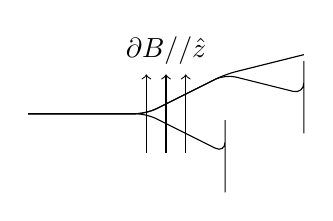
\begin{tikzpicture}
    \draw [rounded corners] (0,0) --++ (1.5,0) --++ (1,.5) --++ (1,.25);
    \draw [rounded corners] (0,0) --++ (1.5,0) --++ (1,.5) --++ (1,-.25) --++ (0,.5) --++ (0,-1);
    \draw [rounded corners] (0,0) --++ (1.5,0) --++ (1,-.5) --++ (0,.5) --++ (0,-1);
    \draw [->] (1.5,-.5) --++ (0,1);
    \draw [->] (1.75,-.5) --++ (0,1) node [above] {$\partial \bm B // \hat z$};
    \draw [->] (2,-.5) --++ (0,1);
  \end{tikzpicture}

  * Only 2 possible outcomes to fixed measurement.

  * Always 2 outcomes by changes measurements, different intensities depend on measurements.
  Orthognal states:
  \begin{itemize}
    \item Projected probability
    \item Measurement (matters!)
  \end{itemize}
\end{itemize}

Math:

Hierarchy of SPACES

Topological space -> Metric space -> Normed vector space -> Inner product space and Bonaic space -> Hilbert space
\begin{itemize}
  \item Topological space: \emph{continuity}
  \item Matrix: Sence of \emph{distance}
  \item Normed vector space (also called linear space): \emph{length} and distance (Linearity)
  \item Bonaic space: Sence of completness (limit / calcules)
  \item Inner product space: Projection/overlap (sence of not only length, but also \emph{angle})
  \item Hilbert space: all of the above.
\end{itemize}

\begin{framed}
  Vector Space
  \begin{framed}
    Inner product space (sometimes called Pre-Hilbert Space)
  \end{framed}
\end{framed}

\section{Vector space}

Vectors (u,v) \& scalors (a,b)
\begin{itemize}
  \item Vector addition ``$+$''
  \fbox{Vectors form abelian group.}
  Abelian group: 4 + 1 properties. (Closure, Identity $\identity$, Inverse (always find another elements, add to it equals to identity), Associatity ($(a+b)+c = a+(b+c)$), Commutativity ($a+b = b+a$))


  \begin{framed}
    Vectors <-> Orthogonal states
  \end{framed}

  \item Scalar multiplication ``$\times$''
  A: Associatity $a(bu) = (ab)u$, I: Identity, Distr
  $f(au+bv) = af(u) + bf(v)$.

  \begin{framed}
    Scalars <->  Projected probability (amplitudes)
  \end{framed}
\end{itemize}

\section{Inner product space}

by adding one more ~: V, F, $\braket<|>$ (Inner product): C(Conjugate symmerty: take two input $\braket<u|v> = \braket<v|u>^*$ for complex number), Li (Linear Reality: $\braket<w|au + bv> = a\braket<w|u> + b\braket<w|v>$), P (Positive definiteness: $\braket<u|v> > 0$ of $u \neq 0$.)

\begin{framed}
  Inner Project <- orthogonal, projected, measurement
\end{framed}

Operators:

Maps on Hilbert Space (linear): $Z: V \to V$

Two important defs:
\begin{itemize}
  \item Operators: compute sth. like $\ab|{\braket<u|\hat O|u>}|$
\end{itemize}

\section{Features of Hilbert space}

\begin{itemize}
  \item Main basis
  \item Maps
\end{itemize}

Hilbert Space naturally describes quantum objects: superposition; complex probability amplitudes;

\fbox{Vector space \fbox{Inner product space} ~ } \kern-1em \textrightarrow $\ket|\psi> = a\ket|u> + b\ket|v>$ \textrightarrow superposition

\fbox{IPS} \textrightarrow $\braket<u|\psi> \leftrightarrow $ complex probability amplitudes.

\begin{definition}[Basis <Mathematical definition>]\leavevmode
  \begin{itemize}
    \item Linear independence
    For a set of vectors $A = \{v_i\}$ in a vector space: If
    \[\sum_A a_i v_i = 0 \Rightarrow \forall a_i = 0\]
    then $A$ is linearly independent.
    \item Linear span:
    $span(A) = \{\sum_A a_iv_i,~ a_i \in F\}$ ($F$: Field, as complex number $F \in \mathbbm C$)

    $E = \{e_i\}$ is a basis of $V$. If
    \begin{itemize}
      \item $\{e_i\}$ is linear independence
      \item $span(\{e_i\}) = V$
    \end{itemize}
    \item Dimension of Vector space: $\dim(V) = card(E)$.
    \item Expansion of $V$ over $E$
    \[
      V = \sum a_i e_i
    \]
    This expansion is unique\footnote{}.
  \end{itemize}
\end{definition}

\begin{definition}[Orthonormal Basis]
  Use $\{\ket|\alpha>\}$ for all orthogonal states, and it satisfies
  \[
    \braket<\alpha|\alpha'> = \delta_{\alpha\alpha'}
  \]
  $\alpha$ is a lable, different labels means different states. If they are different, they are orthogonal.

  Completness condition:
  \[
    \sum_\alpha \ketbra|\alpha><\alpha| = \mathbbm I_V
  \]
  $\mathbbm I$ means identity in the Hilbert space. We call the operators like this the projector $P_\alpha$: projector to the state $\ket|\alpha>$

  Existence / construction: Gram-Schmidt orthognalization.
  $\d i = e_i - \sum_{j < i} p_j e_j$

  Expension over $\{\ket|\alpha>\}$.
  \[
    \ket|\psi> = \sum_\alpha \psi_\alpha \ket|\alpha>
  \]
  \[
    \braket<\alpha|\psi> = \sum_{\alpha '}\psi_{'\alpha'}\braket<\alpha|\alpha'>,~
    \psi_\alpha \in \mathbbm C
  \]
\end{definition}

\begin{example}
  $\alpha \to x$, $\psi_\alpha \to \psi(x)$ wavefunction

  $\alpha \to k$, $\psi(k) = \int \d x \upe^{\iu kx} \psi(x)$

  $\{\alpha\} \to \{0,1\}$, $\psi_\alpha \to (\psi_0, \psi_1)\tran$

  $\ket|0>$, $\ket|1>$.

  $\alpha \to \{(k,\sigma)\}$, $\psi_\alpha \to \psi_\sigma (k)$
\end{example}


\subsection{Change of Basis}

$\{\ket|\alpha>\} \to \{\ket|\beta>\}$

\[
  \ket|\psi> = \sum_\alpha \psi_\alpha \ket|\alpha> = \sum_\beta \psi_\beta \ket|\beta>
\]
\[
  \psi_\beta = \braket<\beta|\psi> = \sum_\alpha \braket<\beta|\alpha>\braket<\alpha|\psi> = \sum_\alpha U_{\beta\alpha} \psi_\alpha.
\]
$\beta \to k$, $\alpha \to x$
\[U_{\beta\alpha} \to \braket<k|x> = \upe^{-\iu kx}\]

\section{Maps}

Maps: just the arrow.

For vector space $(V,F)$ (sth we call vectors and scalors).

%   -> F
% V -> V
%   -> W

% Linearity (linear maps)

From $V$ to $F$: linear function

From $V$ to $V$: linear operator

Linear:

$f: V \to W$

$f(au + bv) = af(u) + bf(v)$
\[
  \{f(\text{linear}):V \to W\} = \text{Hom}_F (V,W) \text{is V.S.}
\]
\fbox{Scalor is just the one Dimension of V.S..}

$f, g \in \mathcal V$. $\forall v \in V$, $(f + g) = f(v) + g(v) \in W$.

For commutativity`', $f \cdot g = g \cdot f \in W$.

\begin{table}[!htbp]
  \centering
  \begin{tabular}{ccc}
    \toprule
    Basis & ON. Basis & Components\\
    \midrule
    $\{f_i, f_i(e_j) = \delta_{ij}\}$ & $\{\braket<\alpha|\cdot>\}$\\
    $\{f_{ij}: f_{ij}(l_n) = e_i\delta_{jk}\}$ & $\{\bra<\alpha|\}$\\
    $\{f_{ij}: f_{ij}(e_k) = e_i'\delta_{jk}\}$ & \\
    \bottomrule
  \end{tabular}
\end{table}
$\braket<\hat F|\hat G> = \sum_\alpha \braket<\hat F_\alpha|\hat G_\alpha>$
and $\hat F\ket|G> = \sum_n \braket<\alpha|\alpha>\bra<G|$
\[
  \bra<F\beta| = \sum_\alpha \braket<\beta|\alpha>\bra<\hat F_\alpha|,~
  F\ket|\beta> = \sum_\alpha \hat F \ket|\alpha>\braket<\alpha|\beta>
\]
with $\sum_\beta \ketbra|\beta><\beta| = \identity$
\[
  \sum_\beta \braket<\hat F\beta|\hat G\beta>
  = \sum_{\beta\alpha\alpha'}\braket<\beta|\alpha>\braket<F\alpha|G\alpha'>\braket<\alpha'|\beta>
\]
Then, we have
\[
  \braket<\hat F|\hat G> = \Tr(F^{-1}G) = \sum_\alpha\braket<F\alpha|G\alpha> = \sum_\alpha \braket<\alpha|F^\dagger G|\alpha>
\]
\[
  \Tr[(\ketbra|\alpha'><\alpha|)^\dagger(\ketbra|\beta><\beta'|)] = \delta_{\alpha\beta}\delta_{\alpha'\beta'}
\]
\[
  \hat O = \sum_{\alpha\beta} \ket|\alpha>\braket<\alpha|\hat O|\beta>\bra<\beta|
  = \sum_{\alpha\beta} O_{\alpha\beta}\ketbra|\alpha><\beta|
\]

How about $V \times V$? --- Inner product, a set of all pairs. It has to BILINEAR.
\[
  f(au+bv,w) = a^*f(u,w) +*b^f(v,w)
\]

$V \times V \to V \otimes V$ ($\otimes$: $V \times V \to V \otimes V$, a map)

\[w = \sum_{ij} W_{ij} (e_i \otimes e_j) = u \otimes v\]
Given $u$ and $v$, what the Components of $u \otimes v$?

Suppose $u$ is written as $u = \sum_i u_i e_i$ and $v$ is written as $v = \sum_j v_j e_j$. Then,
\[
  u \otimes v = \ab(\sum_i u_i e_i) \otimes \ab(\sum_j v_j e_j)
= \sum_i u_i (e_i \otimes \sum_j v_j e_j)
= \sum_{ij} u_iv_j (e_i \otimes e_j)
\]
We start from something like
\[
  w = w_ie_1\otimes e_1 + w_2 e_2 \otimes e_2
\]
which $w_1$ and $w_2$ are both finite.
Suppose $w = u \otimes v$ is true, then
\[
  w = \sum_{ij} u_iv_j (e_i \otimes e_j)
\]
\emph{but we have chosen a specific $w$}, it means that
\[
  w = u_1v_1(e_1 \otimes e_2) + u_1v_2(e_1\otimes e_2) + u_2v_1(e_2\otimes e_1) + u_2v_2(e_2\otimes e_2)
\]
Comparing with $w = w_ie_1\otimes e_1 + w_2 e_2 \otimes e_2$, we have
\[
  w_1 = u_1v_2, ~ 0 = u_1v_2, ~ 0 = u_2v_1, ~ w_2 = u_2v_2
\]

\subsection{Case study: (Re)discover Fourier Transform}

\begin{paracol}{2}
  We've always talk about $\{\ket|\alpha>\}$, but now,
  consider a Hilbert space, label basis $\{\ket|l>\}$ with order number index:
  \[
    \{\ket|l>,\ l = 1,\ 2,\ \ldots\,.~N\}
  \]
  and also we may want to $N + 1 \equiv 1$,
  something like a circle with all the states
  $\ket|1>$, $\ket|2>$, $\ldots\,$,~$\ket|n>$ in the right figure.

  In this basis, we define translation (operator $\hat T_L$)
  \[\hat T_L\ket|l> = \ket|l + 1>,\]
  and we may also write it differently like
  \switchcolumn \centering
  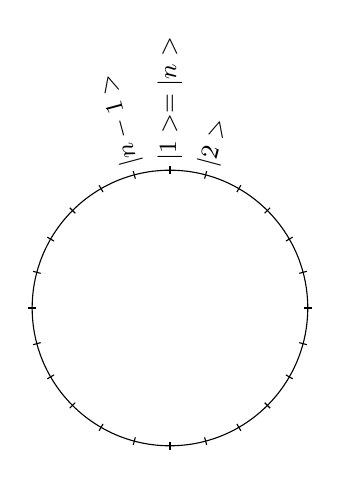
\begin{tikzpicture}[font = \small]
    \draw (0,0) circle (1.75);
    \foreach \i in {15,30,...,360}
      \draw (\i:1.7) --++ (\i:.1);
    \node [right, rotate around = {90:(0,0)}] at (90:1.75) {$\ket|1> = \ket|n>$}
     node [right, rotate around = {75:(0,0)}] at (75:1.75) {$\ket|2>$}
     node [right, rotate around = {105:(0,0)}] at (105:1.75) {$\ket|n - 1>$};
  \end{tikzpicture}
\end{paracol}
\begin{equation}
  \hat T_L = \sum_l \ketbra|l + 1><l|,
\end{equation}
The eigenvalue
\[
  \hat T_L\ket|\psi> = \lambda \ket|\psi>
\]
while $\ket|\psi> = \sum_l \psi_l \ket|l>$, that is
\begin{align*}
  \hat T_L\ket|\psi>  & = \sum_l \psi_{l-1}\ket|l>\\
  \lambda\ket|\psi>   & = \sum_l \lambda \psi_l \ket|l>
\end{align*}
Then we have
\[
  \psi_l = \lambda \psi_l, ~ \psi_l = \lambda^{1-l}\psi_l,~
  \psi_1 = \psi_{N+1} = \lambda^{-N}\psi_1
\]
then we have $\lambda^{-N} = 1$. So, we can specify $\lambda$
\begin{equation}
  \lambda = \lambda_m \equiv \upe^{-\iu \frac{2\pi}Nm}
\end{equation}
Concering the eigenstates of $\hat T_L$, which are $\ket|m>$. Since
\[
  \psi_{1,m} = \lambda_m^{-1}, ~ \psi_{l,m} = \lambda_m^{1-l}\psi_{1,m} = \lambda_m^{-l}
\]
So,
\[
  \ket|m> = \sum_l \psi_{l,m}\ket|l> = \frac1{\sqrt N} \sum\upe^{\iu \frac{2\pi}{N} ml} \ket|l>
\]
Now, consider the new basis ($m = 1$, $2$, $\ldots\,$,~$N$), 
the relation between it and the old basis is
\[
  \{\ket|l>\} \xleftrightarrow{\text{Fourier Transform}} \{\ket|m>\}
\]
In this basis, the definition of the operator is
\begin{equation}
  \hat T_L = \sum_m \upe^{-\iu \frac{2\pi}{N}m} \ketbra|m><m|.
\end{equation}
with $N + 1 \equiv 1$.
and the inner product
\begin{equation}
  \braket<l|m> = \frac1{\sqrt N}\upe^{\iu\frac{2\pi}{N}lm}
\end{equation}
To make the problem more interesting: the translation of the $m$-basis,
express $\hat T_M$ in terms of $l$
\begin{equation}
  \hat T_M = \sum_m \ketbra|m + 1><m|
= \sum_{mll'} \ket|l>\braket<l|m+1>\braket<m|l'>\bra<l|
\end{equation}
If we put $m + 1$ instead of $m$
\[
  \braket<l|m + 1> = \upe^{\iu\frac{2\pi}{N}l} \braket<l|m>
\]
subsitute it into $\hat T_M$
\[
  \hat T_M = \sum_l \upe^{\iu\frac{2\pi}{N}l}\ketbra|l><l|
\]
To summarize
\begin{align}
  \hat T_L & = \upe^{-\iu\frac{2\pi}{N}\hat M}, ~
  \hat M = \sum_m m\ketbra|m><m|\\
  \hat T_M & = \upe^{-\iu\frac{2\pi}{N}\hat L}, ~
  \hat M = \sum_m m\ketbra|l><l|
\end{align}
This is only a start. How about the translation over $m$:
\[
  \hat T_L \hat T_M = \underline? \hat T_M \hat T_L,
\]
means we can measure $M$ first, then measure $L$; or reverse.
They will differ by something like
\[
  \hat T_M \hat T_L = \hat T_L \hat T_M \upe^{\iu\frac{2\pi}{N}}
\]
Comparing with $[\hat q,\hat p] = \iu$.
Just consider in the $l$ basis, expand $\hat T_L$ and $\hat T_M$
\begin{align*}
  \hat T_L \hat T_M & = \sum_{ll'} \ketbra|l + 1><l| \upe^{\iu\frac{2\pi}{N}l'}\ketbra|l'><l'|
= \sum_l \upe^{\iu\frac{2\pi}{N}l}\ketbra|l + 1><l|\\
  \hat T_M \hat T_L & = \sum_{ll'} \upe^{\iu\frac{2\pi}{N}l'} \ket|l'>\braket<l'|l + 1>\bra<l|
= \sum_l \upe^{\iu\frac{2\pi}{N}(l+1)} \ketbra|l + 1><l|
\end{align*}
That is
\begin{equation}
  \hat T_M \hat T_L = \upe^{\iu\frac{2\pi}{N}}\hat T_L \hat T_M
  \label{1.7}
\end{equation}
When $N = 2$: we reach \emph{Ultra Quantum};
When $l = 0$, $1$: $\hat T_M \to \sigma_z$, and $\hat T_L \to \sigma_x$.
We get the anti-commute relation
\begin{equation}
  \sigma_z \sigma_x = -\sigma_x\sigma_z
\end{equation}
When $N \to \infty$, $q = la$ while $a \to 0$,
similarly, $p = mb = m\frac{2\pi}{Na}$. Eventually, $b \to 0$, $N \to \infty$.

Let $\hat Q = \hat La$, $\hat P = \hat Mb$, now
\[
  \hat T_M \to \hat T_Q = \upe^{\iu b\hat Q}, \qq{and}
  \hat T_L \to \hat T_P = \upe^{-\iu a\hat P}
\]
Next, what we need to do is to expand the exponential to linear order: from \eqref{1.7}, we have
\[
  (\identity + \iu b\hat Q) (\identity - \iu a\hat P)
= (\identity + \iu ab) (\identity - \iu a\hat P) (\identity + \iu b\hat Q)
\]
Omit the high order terms, then we have
\begin{equation}
  \hat Q \hat P = \iu + \hat P \hat Q, \qq{or} [\hat Q, \hat P] = \iu
\end{equation}
$Q$ and $P$ are Hermitian Operators.

\noindent\rule{\linewidth}{1pt}

\[
  \hat O\ (V \to V)
  \begin{cases*}
    \text{Invertible:} &
    Symmetry Operators (e.g. projection: $\ketbra|\alpha><\alpha|$ or $\sum_{\{\alpha\}\in \text{H.S.}} \ketbra|\alpha><\alpha|$)\\
    & Transformation, time evolution: Unitary $U^\dagger U = \identity$\\
    \text{Non-Invertible:} & Generators \texttt{<->} Obserables\\
    & Hamiltonian, position \texttt{<->} momentum: Hermitian $O^{-1} = O$
  \end{cases*}
\]
For any $\Psi X \Psi$, the unitary operation should satisfy the following relation
\begin{equation}
  \braket<\hat UX|\hat O\Psi> = \braket<X|\Psi>
\end{equation}
while the Hermitian operator should satisfy
\begin{equation}
  \braket<\hat OX|\Psi> = \braket<X|\hat O\Psi>
\end{equation}
Another kind of unitary: Anti-Unitary \texttt{<-} Anti-Linear

\section{Time Evolution}

\[\ket|\Psi(t)> = \hat U(t,t_0) \ket|\Psi(t_0)>\]
\[
  \braket<\hat O\Psi(t_0)|\hat O\Psi(t_0)> = \braket<\Psi(t_0)|\Psi(t_0)>
\]

The two statements: Operator $\hat O$ satisfies
\begin{itemize}
  \item $\forall \psi$, $\braket<\hat O\psi|\hat O\psi> = \braket<\psi|\psi>$ (Preserve norm)
  \item $\forall X, \psi$, $\braket<\hat OX|\hat O\psi> = \braket<X|\psi>$ 
  (Preserve inner product)
\end{itemize}
Prove that they are equivalent.
\begin{proof}
  Obviously, 2 to 1 is trivial.
  Let $u = X + \Psi$, $V = X + \iu\Psi$, then subsitute them in to the above formulas.
\end{proof}

\subsection{Equation of Motion}

$\hat U$: linear, continous with time.

We need to consider $\epsilon$ time difference, that is somethint like
\[
  \ket|\Psi(t + \epsilon)> = \hat U(t + \epsilon, t) \ket|\Psi(t)>
\]
\[
  \lim_{\epsilon\to0}
  \frac{\ket|\Psi(t+\epsilon)> - \ket|\Psi(t)>}{\epsilon}
= \lim_{\epsilon\to0} \frac{\hat U(t + \epsilon,t) - \hat U(t,t)}{\epsilon} \ket|\Psi(t)>
\]
\[
  \text{LHS} = \odv*{\ket|\Psi(t)>}t, ~
  \lim_{\epsilon\to0} \frac{\hat U(t + \epsilon,t) - \hat U(t,t)}{\epsilon}
= \odv*{}{t} \hat U(t',t)\bigg|_{t'=t} \equiv \frac1{\iu\hbar} \hat H(t)
\]
Finally, we approach the Schr\"odinger Equation
\begin{equation}
  \odv*{\ket|\Psi(t)>}t = \frac1{\iu\hbar} \hat H(t) \ket|\Psi(t)>
\end{equation}
Prove: $\hat g$ is Hermitian
\begin{equation}
  \odv*{\hat U(\theta)}\theta \bigg|_{\theta=0} = \iu \hat g
\end{equation}
while $\hat U(0) = \identity$.
\begin{proof}
  We know that 
  \[\hat U(\epsilon) = \identity + \iu \hat g\epsilon\]
  Since the definition of Hermitian is
  \[
    \braket<\hat OX|\Psi> = \braket<X|\hat O\Psi>,
  \]
  Then plug $\hat U(\epsilon)$ into the definition
  \[
    \braket<\hat U(\epsilon)X|\hat U(\epsilon)\Psi>
  = \braket<X|\psi> + (-\iu\epsilon)\braket<\hat gX|\Psi>
  + (\iu\epsilon)\braket<X|\hat g\Psi> = \braket<X|\Psi>
  \]
  then we have
  \[
    \braket<\hat gX|\Psi> = \braket<X|\hat g\Psi>
  \]
  means that $\hat g$ is Hermitian.
\end{proof}
$\hat g$ is called the generator; \emph{$\hbar$ / Hamiltonian is the generator of time evolution.}
\begin{equation}
  \iu\odv*{\ket|\Psi(t)>}t = \hat H(t) \ket|\Psi(t)>
\end{equation}
$\hat H$ is canonical quantization. Replace $\ket|\psi(t)>$
\begin{equation}
  \iu\odv*{\hat U(t,t_0)}t = \hat H(t) \hat U(t,t_0)
\end{equation}
Given $\hat H(t)$, find $\hat U(t_f,t_i)$. For t-independent $\hat H$, do small steps from $t_i$ to $t_f$ by $\delta t = (t_f - t_i)/N$
\begin{equation}
  \hat U(t_f,t_i) = \hat U(t_f,t_f - \delta t) \hat U(t_f - \delta t, t_f - 2\delta t) \ldots \hat U(t_i + \delta t, t_i)
\end{equation}
When $N \to \infty$, $\delta t \to 0$, that become
\[
  \hat U(t_f,t_i) = \lim_{N\to\infty}  (\identity - \iu \hat H \delta t)^N
= \lim_{N\to\infty} \ab(\identity - \iu \hat H \frac{t_f - t_i}{N})^N
= \upe^{-\iu\hat H(t_f - t_i)}
= \identity + ()\hat H + ()\hat H^2 + \cdots
\]

\subsection{Dyson series}

When it's time-independent, the order doesn't matter.
Now, consider the $t$-dependent case of $\hat H(t)$
\[
  \hat U(t_f,t_i) = \lim_{\delta t\to0}
                    (\identity - \iu \hat H(t_f)\delta t)
                    (\identity - \iu \hat H(t_f - \delta t)\delta t)
                    \cdots
                    (\identity - \iu \hat H(t_i + \delta t)\delta t)
\]
and convert every term into exponential $\upe^{-\iu\hat H(t_i + \delta)\delta t}$, the first term gets $\upe^{-\iu\hat H(t_f)\delta t}$. Multiply all the exponential function, $\upe^{-\iu\int_{t_i}^{t_f} \d t \hat H(t)}$.
\begin{framed}
  Since $\upe^A\upe^B \sim \upe^C$, but $C = A + B + ()[A,B] + \cdots$.
  And a time ordering operator $\mathcal T$ is applied before the exponential.
\end{framed}
Now, rewrite the S.E
\begin{equation}
  \int_{\mathemph{t_i}}^{t_f} \d \hat U(t,\mathemph{t_i})
= \int_{t_i}^{t_f} [-\iu\hat H(t)] \hat U(t,t_i) \d t
\end{equation}
since the lower limit of the integral $t_i$
and the second time variable of $\hat U$: $t_i$ conduct an identity, that is
\[
  \text{LHS} = \hat U(t_f,t_i) - \hat U(t_i,t_i) = \hat U(t_f,t_i) - \identity
\]
so
\begin{align*}
  \hat U(t_f,t_i) & = \identity + \int_{t_1}^{t_f} \d t_1
                    [-\iu \hat H(t)] \hat U(t_1,t_i)\\
& = \identity + \int_{t_1}^{t_f} \d f_1 (-\iu \hat H(t_1))
  + \int_{t_i}^{t_f} \d t_1 (-\iu \hat H(t_1)) \int_{t_i}^{t_1} \d t_2
    (-\iu\hat H(t_2))\\
& + \cdots + \int_{t_i}^{t_f} \d t_1 + \int_{t_i}^{t_1} \d t_2 \cdots
  + \int_{t_i}^{t_{n-1}} \d t_n (-\iu \hat H(t_1)) \cdots (-\iu\hat H(t_N)) + \cdots
\end{align*}
That's what we called the \emph{Dyson's Series}.
Now, let's take a look at $N$'s order term
\begin{multline}
  \int_{t_i}^{t_f} \d t_1
  \int_{t_i}^{\mathemph{t_1}} \d t_2
  \cdots
  \int_{t_i}^{\mathemph{t_{n-1}}} \d t_n
  \hat H(t_1) \hat H(t_2) \cdots \hat H(t_n)
= \int_{t_i}^{t_f} \d t_1
  \int_{t_i}^{\mathemph{t_f}} \d t_2
  \int_{t_i}^{\mathemph{t_f}} \d t_n\\
  \theta(t_1 - t_2) \cdots \theta(t_{n-1} - t_n)
  \hat H \cdots \hat H
\end{multline}
while
\begin{equation}
  \theta(x) =
  \begin{cases}
    1, & x > 0\\
    0, & x < 0
  \end{cases}
\end{equation}
is the Heaviside Stage Function. It could
\begin{equation}
  \int_{x_0}^{x_1} \d x = \int_{x_0}^{\infty} \d x \theta(x_0 - x)
\end{equation}
\begin{center}
  \begin{tikzpicture}
    \draw (0,0) node [below] {$x_0$} -- (2,0) node [below] {$x_1$} -- (5,0)
     node [below] {$\infty$};
  \end{tikzpicture}
\end{center}
$t_1$, $t_2$, $\ldots$, are Dummy variables.
Then, sum over all of the  permutations
\begin{align*}
  & \int_{t_i}^{t_f} \d t_1
  \int_{t_i}^{\mathemph{t_f}} \d t_2
  \int_{t_i}^{\mathemph{t_f}} \d t_n
  \theta(t_1 - t_2) \cdots \theta(t_{n-1} - t_n)
  \hat H \cdots \hat H\\
  = & \frac1{n!} \sum_\sigma
  \int_{t_i}^{t_f} \d t_{\sigma_1}
  \int_{t_i}^{t_f} \d t_{\sigma_2}
  \cdots
  \int_{t_i}^{t_f} \d t_{\sigma_n}
  \theta(t_{\sigma_1} - t_{\sigma_2}) \cdots
  \theta(t_{\sigma_{n-1}} - t_{\sigma_n})
  \hat H(t_{\sigma_1}) \cdots
  \hat H(t_{\sigma_n})\\
  = & \frac1{n!}
  \int_{t_i}^{t_f} \d t_1
  \int_{t_i}^{t_f} \d t_2
  \cdots
  \int_{t_i}^{t_f} \d t_{\sigma_n} \sum_\sigma[
  \theta(t_{\sigma_1} - t_{\sigma_2}) \cdots
  \theta(t_{\sigma_{n-1}} - t_{\sigma_n})
  \hat H(t_{\sigma_1}) \cdots
  \hat H(t_{\sigma_n})]\\
\equiv & \mathcal T[\hat H(t_1) \cdots \hat H(t_n)]
= \mathemph{\frac1{n!} \mathcal T \ab[\int_{t_i}^{t_f} \d t \hat H(t)]^n}
\end{align*}
while $\sigma: \{1,2,\ldots,n\} \to \{1,2,\ldots,n\}$ is called permutation:
E.g., $\sigma_2$: $1$, $2$, $3 \to 3$, $1$, $2$.
And we introduced the time ordering operator $\mathcal T$ to prevent a Hamiltonian operator with an latter time $\hat H(t_j)$
``knocked'' on $\ket|\Psi(t)>$ earlier that
a Hamiltonian operator with an earlier time $\hat H(t_i)$ will ``knock on'':
that is
$\hat H(t_i) \hat H(t_j) \ket|\Psi(t)>$.

\section*{Review: Time Evolution}

The Schr\"odinger equation
\begin{equation}
  \iu \odv*{\ket|\psi(t)>}t = \hat H(t) \ket|\psi(t)>
\end{equation}
and we can rewrite it in terms of time-evolution operator
\begin{equation}
  \iu \odv*{\hat U(t,t_0)}t = \hat H(t) \hat U(t,t_0)
\end{equation}
and initially, we can write
\[
  \hat H(t) = \iu \odv*{\hat U(t',t)}t \bigg|_{t'=t}
= \iu \ab[\odv*{\hat U(t,t_0)}t] \hat U^{-1}(t,t_0)
\]
the bracket can be generalize something like
\begin{equation}
  \hat g_\theta = \iu \odv*{\hat U(\theta)}\theta \bigg|_{\theta=0}
\end{equation}
and we can have the identity
\begin{equation}
  \hat U(0) = \identity
\end{equation}
In general, the expression of the time-evolution operator is something like
\[
  \hat U(t,t_0) = \mathcal T \upe^{-\iu \int_{t_0}^t \d t' \hat H(t)}
\]
The time-ordering operator is inserted since
\[\upe^A \upe^B = \upe^C \neq \upe^{A+B}\]
BCH formula will tell how to write $C$:
\[
  C = A + B + \frac12[A,B] + \cdots
\]
The time-ordering operator can be also separate into two cases
\[
  \begin{cases*}
    \hat U(t,t_0) = \upe^{-\iu (t-t_0) \hat H}, & time-independent\\
    \hat U(t,t_0) = \identity + (-\iu) \int_{t_0}^t \d t_1 \hat H(t_1)
                  + (-\iu) \int_{t_0}^t \d t_1 \int_{t_0}^{t_1} \d t_2
                    \hat H(t_1) \hat H(t_2) + \cdots, & time-dependent
  \end{cases*}
\]

\subsection{Three Pictures}

Considering representation, the basis $\{\ket|\alpha>\}$.
and in state and operator
\begin{gather}
  \ket|\psi> = \sum_\alpha \psi_\alpha \ket|\alpha>\\
  \hat O = \sum_{\alpha\beta} \hat O_{\alpha\beta} \ketbra|\alpha><\beta|
\end{gather}
where $\psi_\alpha = \braket<\alpha|\psi>$ and $O_{\alpha\beta} = \braket<\alpha|\hat O|\beta>$.

\begin{itemize}
  \item Schr\"odinger: $\{\ket|\alpha>^S = \ket|\alpha>\}$, where $\ket|\alpha>$ is const in time.
  \[
    \odv*{\psi_\alpha^s(t)}t = \odv*{^s\braket<\alpha|\psi(t)>}t
  = (-\iu) ^s\braket<\alpha|\hat H(t)|\psi(t)> = \sum_\beta (-\iu) H_{\alpha} (t) \psi_\beta^s (t)
  \]
  when $\alpha \to x$, $\psi_\alpha(t) = \psi(x,t)$
  \[
    \iu \pdv*{\psi(x,t)}t = \int \d x' H(x,x',t) \psi(x',t)
    \to H(x,-\iu\pdif x, t) \psi(x,t)
  \]
  the propotion $H(x,x',t) $ is something like $\delta(x - x')$.
  \item Heisenberg
  \[
    \{\ket|\alpha(t)>^H = \hat U(t,t_0) \ket|\alpha(t_0)>\}
  \]
  for the state,
  \begin{equation}
    \odv*{\psi_\alpha^H(t)}t = \odv*{^H\braket<\alpha(t)|\psi(t)>}t = 0
  \end{equation}
  means the state is not moving at all.
  Assume $\alpha(t_0) = \alpha$, $\hat U(t,t_0) = \hat U(t)$, and $\psi(t_0) = \psi$.
  \[
    \odv*{O_{\alpha\beta}^H(t)}t = \odv*{^H\braket<\alpha(t)|\hat O|\beta(t)>^H}t = \odv*{\braket<\alpha|\hat U^{-1}(t) \hat O \hat U(t)|\beta>}t
  \]
  where $\hat U^{-1}(t) \hat O \hat U(t) = \hat O^H(t)$. Then
  \[
    \odv*{\hat O^H(t)}t = \odv*{(O^{-1}(t) \hat O \hat U(t))}t
  \]
  where $\odv*{\hat U^{-1}(t)}t = \iu \hat U^{-1}(t) \hat H(t)$.
  Finally, we have
  \begin{equation}
    \odv*{\hat O^H(t)}t = \iu[\hat H^H(t), \hat O^H(t)]
  \end{equation}
  which is so called the Heisenberg equation (EOM), where
  \[
    \hat H^H(t) = \hat U^(t)^{-1} \hat H(t) \hat U(t)
  \]
  \item Interaction
  
  We have two part of Hamiltonian
  \[
    \hat H = \hat H_0 + \hat V
  \]
  what is important is that $\hat H_0$ is the easy part,
  we can easily compute the time evolution $\hat U_0(t)$.
  Then, the basis will be chosen as
  \[
    \{\ket|\alpha(t)>^I = \hat U_0(t) \ket|\alpha>\}
  \]
  then
  \begin{equation}
    \odv*{\psi_\alpha^I(t)}t = \odv*{^I\braket<\alpha(t)|\psi(t)>}t
  = \odv*{\braket<\alpha|\hat O^{-1} \hat U(t)|\psi>}t.
  \end{equation}
  and we consider $\hat O^{-1} \hat U(t)\ket|\psi> = \ket|\psi(t)>^I$.
  Similarly,
  \begin{align*}
    \odv*{\ket|\psi_\alpha(t)>^I}t &
  = \iu \hat U_0^{-1} (\hat H_0(t) - \hat H(t)) \hat U(t) \ket|\psi>
  = \odv*{(\hat U_0^{-1} \hat U(t) \ket|\psi>)}t (?)\\ &
  = -\iu \hat U_0^{-1}(t) \hat V(t) \hat U_0(t) \hat U_0^{-1}(t) \hat V(t) \ket|\psi>
  = -\iu \hat V^I(t) \ket|\psi(t)>^I
  \end{align*}
  where $\hat U_0^{-1}(t) \hat V(t) \hat U_0(t) = \hat V^I(t)$ and
  $\hat U_0^{-1}(t) \hat V(t) \ket|\psi> = \ket|\psi(t)>^I$,
  and $\hat O(t) = \hat U_0^{-1}(t) \hat O \hat U_0(t)$.
  \[
    \odv{\hat O^I(t)}t = \iu [\hat H_0^I(t), \hat O^I(t)]
  = \odv*{(\hat U_0^{-1}(t) \hat O \hat U_0(t))}t
  \]
\end{itemize}

\hrule

\paragraph{Quiz 4}

\begin{problem}
  Given
  \[
    \odv*{\hat U_0(t,t_0)}t = -\iu \hat H_0(t) \hat U_0(t,t_0),
  \]
  show that
  \[
    \odv*{\hat U_0^{-1}(t,t_0)}t = \iu \hat U_0^{-1}(t,t_0) \hat H_0(t).
  \]
\end{problem}
\begin{solution}
  
\end{solution}

\begin{problem}
  Given
  \[
    f(z) = \upe^{-\frac12(x-z)^2}, \quad (x \in \mathbb R,~ z \in \mathbb C)
  \]
  compute
  \[
    \int_{-\infty}^{+\infty} |f(x)|^2 \d x.
  \]
\end{problem}
\hrule

\subsection{Case study}

\begin{enumext}[wrap-label = \underline{Case #1}, label = \arabic*,
                list-indent = 0pt]
  \item Quantum Harmonic Oscillator\\
  Certainly, this is a time-independent problem, the Hamiltonian is given as
  \[
    \hat H = \frac{\hat p^2}{2m} + \frac12 m\omega^2 \hat X^2.
  \]
  For simplifaction, we define $l_0 = \sqrt{\frac\hbar{m\omega}}$, then
  \[
    \hat X = \frac{\hat x}{l_0}, \qq{and} \hat k = \frac{\hat p l_0}\hbar.
  \]
  So, the original commutation relation becomes
  \[
    [\hat x, \hat p] = \iu\hbar \longrightarrow [\hat x, \hat k] = \iu.
  \]
  Certaily, we need
  \[
    \hat a = \frac1{\sqrt2} (\hat x + \iu\hat k), \qq{and}
    [\hat a, \hat a^\dagger] = 1
  \]
  and let $\hbar = 1$. Then
  \[
    \hat H = \omega(\hat a^\dagger \hat a + \frac12)
  \]
  where $\hat a^\dagger \hat a = \hat N$, the number operator.
  \begin{enumext}
    \item The eigenstates
    $\ket|n> = \frac1{\sqrt{n!}} (\hat a^\dagger)^n \ket|0>$, and
    $\hat a \ket|0> = 0$.
    Consider
    \[
      \ket|n(t)> = \hat U(t) \ket|n> = \upe^{-\iu\omega(n+\frac12)t} \ket|n>
    \]
    Then
    \[
      \braket<n(t)|\hat x|n(t)> = 0, \qq{and} \braket<n(t)|\hat k|n(t)> = 0
    \]
    where
    \[
      \hat x = \frac1{\sqrt2}(\hat a + \hat a^\dagger),
      \hat k = \frac1{\sqrt2\iu} (\hat a - \hat a^\dagger)
    \]
    In Heisenberg picture
    \[
      \dot{\hat x}(t) = \iu[\hat H(t), \hat x(t)] = \omega \hat k(t), \qq{and}
      \dot{\hat k}(t) = \iu[\hat H, \hat k(t)]    = -\omega \hat x(t)
    \]
    and we have
    \[
      \dot{\hat a}(t) = -\iu\omega\hat a(t) \Rightarrow
      \hat a(t) = \upe^{-\iu\omega t} \hat a
    \]
    \[
      \hat x(t) =  \cos\omega t \hat x + \sin\omega t \hat k,
      \hat k(t) = -\sin\omega t \hat x + \cos\omega t \hat k.
    \]
    \item Coherent States $\{\ket|\alpha>\}$
    \begin{gather*}
      \hat a \ket|\alpha> = \alpha \ket|\alpha>, ~ \alpha \in \mathbb C\\
      \ket|\psi> \sim \sum_\alpha \psi_\alpha \ket|\alpha>,~ 
      \ket|\psi(t)> = \sum_\alpha \psi_\alpha \ket|\alpha(t)>\\
      \hat a(-t) \ket|\alpha(t)> = \alpha \ket|\alpha(t)>,~
      \hat U^{-1} \hat a \hat I^{-1}(-t) \hat U(t) \ket|\alpha>\\
      \upe^{\iu\omega t} \hat a\ket|\alpha(t)> = \alpha \ket|\alpha(t)>
      \Rightarrow \alpha(t) = \upe^{-\iu\omega t} \alpha
    \end{gather*}
    What if $\ket|x(t)>$, or in other words $\ket|\psi>$ is $\ket|x_0>$
    \[
      \braket<\alpha|x_0> = \int_{x_0} (\alpha)
    \]
    \[
      \ket|\alpha> = \sum_n^\infty f_{\alpha,n} \ket|n>
    \]
    while
    \[
      \hat a\ket|\alpha> = \sum_n f_{\alpha,n} \sqrt n \ket|n - 1>
    = \sum_n f_{\alpha, n+1} \ket|n>
    \]
    where
    \[
      f_{\alpha, n+1} = \frac{\alpha}{\sqrt{n+1}} f_{\alpha,n},
      \quad
      f_{\alpha.n} = \frac{\alpha^n}{\sqrt{n!}} f_{\alpha,0}
    \]
    and
    \[
      \ket|\alpha> = N \sum_n \frac{\alpha^n}{\sqrt{n!}} \ket|n> = N \upe^{\alpha} a^{n-1} \ket|0>, \quad \ket|n> = ...
    \]
    Concering $\braket<x|\alpha>$: since
    \[
      \alpha f_\alpha(x) = \braket<x|\hat a|\alpha>
    = \int \d x' \braket<x|\hat a|x'> \braket<x'|\alpha>
    \]
    substitute $\hat a = \frac1{\sqrt 2} (\hat x + \hat k)$
    \[
      \alpha f_\alpha(x) = \frac1{\sqrt2} (x + \pdif x) f_\alpha(x)
    \]
    and
    \[
      f_\alpha(x) = N \upe^{-\frac12(x - \sqrt 2a)^{\frac\alpha2}}
    \]
    where $|f_\alpha(x)|^2 = \frac1{\sqrt\pi}\upe^{-(x-\sqrt2\alpha_x)^2}$
  \end{enumext}
  \item Rabi Problem\\
  The Hamiltonian
  \[
    \hat H(t) =
    \begin{pmatrix}
      \frac\Omega2 & \gamma\upe^{-\iu\omega t}\\
      \gamma \upe^{\iu\omega t} & -\frac\Omega2
    \end{pmatrix}
  \]
  bascially time-dependent.
  $\frac\Omega2$ and $-\frac\Omega2$ means the gap between $\ket|0>$ and
  $\ket|1>$ is $\Omega$; and driver frenquency $\omega$, intensity $\gamma$.
  \[
    U(t) =
    \begin{pmatrix}
      \ket|0> \to \ket|0> & \ket|1> \to \ket|0>\\
      \ket|0> \to \ket|1> & \ket|1> \to \ket|1>
    \end{pmatrix}
  \]
  Compute $H_0 = \pdiagmat{\frac\omega2, -\frac\omega2}$.

  Firstly, the definiton of $U_0(t)$.
  Normally, $U_0(t) = \upe^{-\iu tH_0}$; In this case
  \[
    U_0(t) = \pdiagmat{\upe^{-\iu\frac\omega2t}, \upe^{\iu\frac\omega2t}}
  \]
  and
  \[
    U_0^{-1}(t) H(t) U_0(t)
  = \begin{pmatrix}
      \frac\Omega2 & \gamma \\ \gamma & -\frac\Omega2
    \end{pmatrix},~
    V =
    \begin{pmatrix}
      \frac{\Omega - \omega}2 & \gamma\\
      \gamma & -\frac{\Omega - \omega}2
    \end{pmatrix}
  \]
  We get a matrix equation
  \[
    \iu \odv*{U(t)}t = V U(t)
  \]
  the solution is
  \[
    U(t) = \cos Delta_\omega t - \iu \sin\Delta_\omega t
    \ab(\cos\theta_\omega \sigma_z + \sin \theta_\omega \sigma_x)
  \]
  where
  \[
    \Delta_\omega = \sqrt{\ab(\frac{\Omega - \omega}{2})^2 + r^2}, \quad
    \tan \theta_\omega = \frac{2\gamma}{\Omega - \omega}
  \]
  and
  \[
    P_{0\to1}(t) = \frac{\gamma^2}{\ab(\frac{\Omega - \omega}{2})^2 + \gamma^2} \sin^2(\Delta_\omega t)
  \]
  probability: Center: $\Omega$, and $\gamma$ (coupling strength), giving a width. It's very small, means the peek is sharp;
  If $\gamma$ is large, ...
\end{enumext}
% !TeX root = ../main.tex

\chapter{Path Integral}

\begin{enumext}[label = *]
  \item What is a path? --- $x(t)$.
  $\phi: I \equiv [0,1] \to R^d$, $t \in I$, $t_i = 0$, $t_f = 1$.
  
  $I \to R^d$, $I \to M$, $R^{d+1} \to M$: $\phi \in$ Function space.
  ($d + 1$: dimension and time)
  \item What to integrate? $\sum_\phi G[\phi]$. $G: V \to \mathbb C$.

  E.g.: $F[x(t)] \to f(x_1,x_2, \cdots x_N) \leftarrow f(x) = ax^m $
  \item Quantization Schemes: Canonical Quantization $\Leftrightarrow$ Path Integral

  States \& Operators.

  In qm, $\braket<O_1,O_2> \to$ trasition amplitudes, propagate.

  Something like $\int \mathcal D\phi G[\phi]$ will eventually produce something like $\braket<O_1,O_2>$.
\end{enumext}

\section{Compare Quantum with Classical Limit}

\begin{enumext}[label = (\alph*)]
  \item Quantum
    \[
      \hat U(t_f,t_i) = \mathbbm 1 + \ab(-\frac\iu\hbar) \int_{t_i}^{t_f} \d t_1 \hat H(t_1)
    + \ab(-\frac\iu\hbar)^2 \int_{t_i}^{t_f} \d t_1 \int_{t_i}^{t_1} \d t_2   \hat H(t_1) \hat H(t_2) + \cdots
    \]
    Problem: Discontinuous!
    The Hamiltonian actually shall be ``local''.
    One of $H$ act on state, it could not jump.
    \begin{center}
      \begin{minipage}{.42\linewidth}
        \centering
      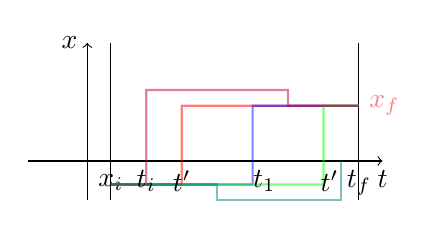
\begin{tikzpicture}[xscale = 1.5]
        \draw (.2,-.5) node [ above ] {$x_i$} --++ (0,2);
        \draw (2.3,-.5) --++ (0,2);
      \draw [->] (-.5,0) -- (2.5,0) node [below] {$t$};
      \draw [->] (0,-.5) -- (0,1.5) node [left] {$x$};
      \draw [thick, opacity = .5, red] (.2,-.3) --++ (.6,0) --++ (0,1) -- (2.3,.7) node [right] {$x_f$};
      \draw [thick, opacity = .5, blue] (.2,-.3) --++ (1.2,0) --++ (0,1) -- (2.3,.7);
      \draw [thick, opacity = .5, green] (.2,-.3) --++ (1.8,0) --++ (0,1) -- (2.3,.7);
      \draw [thick, opacity = .5, purple] (.2,-.3) --++ (.3,0) --++ (0,1.2) --++ (1.2,0) --++ (0,-.2) -- (2.3,.7);
      \draw [thick, opacity = .5, teal] (.2,-.3) --++ (.9,0) --++ (0,-.2) --++ (1.05,0) --++ (0,.5);
      \node [below] at (.5,0) {$t_i$}
       node [below] at (.8,0) {$t'$}
       node [below] at (1.5,0) {$t_1$}
       node [below] at (2.05,0) {$t'$}
       node [below] at (2.3,0) {$t_f$};
      \end{tikzpicture}
      \end{minipage}
      \hspace*\fill
      It should be
      \hspace*\fill
      \begin{minipage}{.42\linewidth}
        \centering
      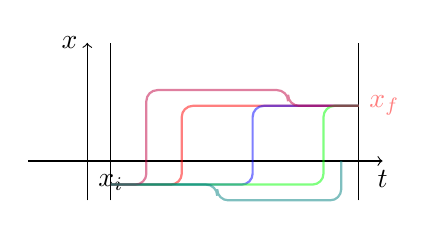
\begin{tikzpicture}[xscale = 1.5]
        \draw (.2,-.5) node [ above ] {$x_i$} --++ (0,2);
        \draw (2.3,-.5) --++ (0,2);
      \draw [->] (-.5,0) -- (2.5,0) node [below] {$t$};
      \draw [->] (0,-.5) -- (0,1.5) node [left] {$x$};
      \draw [rounded corners, thick, opacity = .5, red] (.2,-.3) --++ (.6,0) --++ (0,1) -- (2.3,.7) node [right] {$x_f$};
      \draw [rounded corners, thick, opacity = .5, blue] (.2,-.3) --++ (1.2,0) --++ (0,1) -- (2.3,.7);
      \draw [rounded corners, thick, opacity = .5, green] (.2,-.3) --++ (1.8,0) --++ (0,1) -- (2.3,.7);
      \draw [rounded corners, thick, opacity = .5, purple] (.2,-.3) --++ (.3,0) --++ (0,1.2) --++ (1.2,0) --++ (0,-.2) -- (2.3,.7);
      \draw [rounded corners,  thick, opacity = .5, teal] (.2,-.3) --++ (.9,0) --++ (0,-.2) --++ (1.05,0) --++ (0,.5);
      \end{tikzpicture}
      \end{minipage}
    \end{center}
    $U$ can be decompose like
    \[
      \hat U(t_f,t_i) = \hat U(t_f,t_{N-1}) \cdots \hat U(t_N,t_{N-1}) \cdots \hat U(t_i,)
    \]
    \item Path Integral
    \begin{align*}
      & U(x_f,t_f;x_i,t_i) \equiv \braket<x_f|\hat U(t_f,t_i)|x_i>\\
    = & \int \d x_i \cdots \d x_{N-1} \braket<x_f |\hat U(t_f,t_{N-1})|x_{N-1}>
    \braket<x_{N-1}|\hat U(t_{N-1},t_{N-2})|x_{N-2}> \cdots\\
    & \braket<x_n |\hat U(t_n,t_{n-1})|x_{n-1}> \cdots \braket<x_1|\hat U(t_1,t_i)|x_i>
    \end{align*}
    Basically, we can write the time evolution
    \[
      U(x_n,t_n;x_{n-1},t_{n-1}) = \braket<x_n |\hat U(t_n,t_{n-1})|x_{n-1}> \approxeq \braket<x_n|\upe^{-\frac\iu\hbar\hat H(t_n) \delta t}|x_{n_1}>
    \]
    it's vavid when $\delta t$ is very small.
    Insert a complete basis
    \begin{align*}
      U(x_n,t_n;x_{n-1},t_{n-1}) & \approxeq
      \int \d p_n \braket<x_n|\upe^{-\frac\iu\hbar\hat H(t_n) \delta t}|p_n>\braket<p_n|x_{n_1}>\\
      & = \frac1{2\pi\hbar} \int \d p_n \upe^{\frac\iu\hbar}[p_n(x_n - x_{n-1}) - H(x_n,p_n,t_n)\delta t]
    \end{align*}
  Consider
  \[
    \int \prod_{n=1}^{N-1} \d x_n \int\prod_{n=1}^N \d p_n
  \]
  which is so called ``path'': in phase space path integral.
  (Consider the time is divided in many pieces).
  Then $U(x_n,t_n;x_{n-1},t_{n-1})$ can be
  \[
    U(x_n,t_n;x_{n-1},t_{n-1}) = \int \d p_n \upe^{\frac{\iu}{\hbar} [p_n\dot x_n - \frac{p_n^2}{2m} - V(x_n,t_n)]\delta t}
  = \ab(\frac m{2\pi\iu\hbar\delta t})^{1/2} \upe^{\frac\iu\hbar[\frac12m\dot x_n^2 - V(x_n,t_n)]\delta t}
  \]
  where $\dot x_n = \frac{x_n - x_{n-1}}{\delta t}\big|_{\delta t \to 0}$,
  and $\frac12m\dot x_n^2 - V(x_n,t_n)$ is the Lagrangian $\mathcal L(x_n,\dot x_n,t_n)$.
  Eventually,
  \[
    U(x_f,t_f;t_i,t_i) = \ab(\frac m{2\pi\iu\hbar\delta t})^{N/2}
    \int \prod_{n=1}^{N-1} \d x_n \upe^{\frac\iu\hbar \sum_{n=1}^{N-1}}
    \mathcal L(x_n,\dot x_n,t_n) \delta t
  = \int \mathcal D x(t) \upe^{\frac\iu\hbar\mathcal S[x]}
  \]
  where $\mathcal D = \int \prod_{n=1}^{N-1} \d x_n$,
  and $\mathcal S[x] \equiv \int_{t_i}^{t_f} \d t \mathcal L(x,\dot x,t)$ ($N \to \infty$).
  In summary, we obtain
\begin{equation}
  U(x_f,t_f;x_i,t_i) \equiv \int \mathcal D x(t) \upe^{-\frac\iu\hbar \mathcal S[x(t)]}
\end{equation}
  where $x(t_i) = x_i$ and $x(t_f) = x_f$.
  \item Classical
  \[
    \hat H(t_n) = \frac{\hat p^2}{2m} + V(\hat x,t_n)
  \]
  Using $\upe^{-\iu\hat H\delta t} \approxeq 1 - \iu\hat H\delta t$.
  Then, we can simply evalute $\braket<x_n|\hat H|p_n>$.
  \[
    \braket<x_n|\upe^{-\frac\iu\hbar\hat H(t_n)\delta t}|p_n>
  = \upe^{-\frac\iu\hbar H(x_n,p_n,t_n)\delta t} \braket<x_n|p_n>
  = \upe^{-\frac\iu\hbar H(x_n,p_n,t_n)\delta t + \frac\iu\hbar p_nx_n}
  \]
  where $H(x_n,p_n,t_n) = \frac{p_n^2}{2m} + V(x_n,t_n)$.
  \hrule \newpage
  Principle of Least Action, EOM determines $x_c(t)$.
  The equation can be derived by
  \begin{equation}
    \delta \mathcal S = 0,\qq{or} (\delta_x\mathcal S)[\eta] = 0, \forall \eta
  \end{equation}
  we fix the initial $(x_i,t_i)$ and the final $(x_f,t_f)$. Consider the other path $x'(t)$, the different is $\eta(t)$.
  Starting from the action
  \begin{equation}
    \mathcal S[x(t)] = \int_{t_i}^{t_f} \d t \mathcal L(x(t), \dot x(t), t)
  \end{equation}
  On another path, the action is
  \[
    \mathcal S[x_c + \eta_c] = \int_{t_i}^{t_f} \d t \mathcal L(x_t + \eta_t, \dot x_t + \dot \eta_t,t)
  = \int_{t_i}^{t_f} \d t \ab[\mathcal L(x_t,\dot x_t,t) + \pdv{\mathcal L}{x_t} \eta t
  + \pdv{\mathcal L}{\dot x_t} \dot \eta_t + \mathcal O(\eta^2)]
  \]
  where
  \[
    \int_{t_i}^{t_f} \d t \ab(\pdv{\mathcal L}{x_t} \eta t
  + \pdv{\mathcal L}{\dot x_t} \dot \eta_t)
  \]
  is so-called \emph{functional derivative}\footnote{From functional space to functional space: $V^* \to V^*$.}: $(\delta_x \mathcal S)[\eta]$.
  Apply the partition integration
  \[
    (\delta_x\mathcal S)[\eta] = \pdv L{\dot x_t} \eta_t \big|_{t_i}^{t_f}
  + \int_{t_i}^{t_f} \d t\ab(\pdv{\mathcal L}{x_t} - \odv*{\pdv{\mathcal L}{\dot x_t}}t)\eta_t
  \]
  since $\eta(t_i) = \eta(t_f) = 0$, so
  \[
    (\delta_x\mathcal S)[\eta] = \int_{t_i}^{t_f} \d t\ab(\pdv{\mathcal L}{x_t} - \odv*{\pdv{\mathcal L}{\dot x_t}}t)\eta_t
  \]
  the integral kernel can be converted to
  \[
    \ab(\pdv{\mathcal L}{x_t} - \odv*{\pdv{\mathcal L}{\dot x_t}}t)\eta_t
  = \braket<\pdv{\mathcal S}{x_i}|\eta>
  \]
  \underline{For $\forall \eta$}, the integral kernel should be zero
  \begin{equation}
    \pdv{\mathcal L}{x_t} - \odv*{\pdv{\mathcal L}{\dot x_t}}t = 0
  \end{equation}
  it's so-called the \emph{Euler-Lagrangian Equation}.
\end{enumext}

Let's talk more about functional derivative.
\[
  (\delta^{(n)}_x\mathcal S)[\eta] = \odv[n]{\mathcal S[x(t) + \epsilon\eta(t)]}\epsilon\bigg|_{\epsilon=0}
\]
the $x$ is supposed to ``where we take the derivative''.
$\mathcal S[x(t) + \epsilon\eta(t)]$ gives a number, but the number is depend on $\epsilon$. So we can define
\[
  \odv[n]{f_{x,\eta}(\epsilon)}{\epsilon} = \mathcal S[x(t) + \epsilon\eta(t)]
\]
\textbf{Quiz}.
Let's try an example.
\[
  \mathcal L(x(t), \dot x(t)) = \frac12m\dot x^2 - \frac12 m\omega^2x^2
\]
Try to find $\delta_x^{(0)}\mathcal S[\eta]$,
$\delta_x^{(1)}\mathcal S[\eta]$,
$\delta_x^{(2)}\mathcal S[\eta]$,
$\delta_x^{(3)}\mathcal S[\eta]$
using the definition.
(Solution: $\delta_x^{(0)}\mathcal S[\eta] = \mathcal S[x]$,
$\delta_x^{(1)}\mathcal S[\eta]$: $\ddot x = -\omega^2t$, $\delta_x^{(2)}\mathcal S[\eta] = 2\mathcal S[\eta]$, $\delta_x^{(> 2)}\mathcal S[\eta] = 0$.)

Let's try to write the Taylor expression of $\mathcal S[x + \eta]$
\begin{equation}
  \mathcal S[x + \eta] = \mathcal S[x + \eta]\big|_{\epsilon = 1} = f(\epsilon)_{x,\eta},
\end{equation}
then, just expand $f(\epsilon)_{x,\eta}$
\[
  \mathcal S[x + \eta] = f(0) + f'(0)\epsilon + \cdots + \frac1{n!}f^{(n)}(0) \epsilon^n + \cdots
\]
Concering $f^{(n)}_{x,\eta} = (\delta_x^{(n)} \mathcal S)[\eta]$, then
\begin{equation}
  \mathcal S[x + \eta] = (\delta^{(0)}\mathcal S)[\eta] + (\delta^{(1)}\mathcal S)[\eta] + \cdots + \frac1{n!}(\delta^{(n)}\mathcal S)[\eta]
= \ab(\upe^{\delta_x}\mathcal S)[\eta]
\end{equation}
\fbox{$\text{ELE} \to x_i(t)$}
\begin{equation}
  \upe^{\frac\iu\hbar\mathcal S[x+\eta]} = \upe^{\frac\iu\hbar(\mathcal S[x] + (\delta_x^{(0)}\mathcal S)[\eta] + \frac12(\delta_x^{(1)}\mathcal S)[\eta] + \cdots)}
\end{equation}
Since $\int \mathcal D\eta(t)$ taken the first order, then the other terms should vanish.
Since classical limit require $\hbar$ to be small.

\section{PI \& Sta. Mech.}

\paragraph{Review}
Starting from propagator
\[
  \braket<x_f|\hat U(t_f, t_i)|x_i> = \sum_{x(t)} \upe^{\iu S[x(t)]}
\]
Summing over all the functions (paths).
This is precisely the quantum interference
\begin{center}
  \begin{tikzpicture}
    \draw (0,0) node [below] {$t_i$} --++ (0,2) node [midway, left] {$x_i$};
    \draw (4,0) node [below] {$t_f$} --++ (0,2) node [near end, right] {$x_f$};
  \end{tikzpicture}
\end{center}
We can use a fancier symbol
\[
  \braket<x_f|\hat U(t_f, t_i)|x_i>
= \int_{x(t_{i,f}) = x_{i,f}} \mathcal D x(t) \upe^{\iu S[x(t)]}
\]
\paragraph{Statistics Mechanics}

Starting from the partition function
\begin{equation}
  Z = \sum_n \upe^{-\beta E_n} = \sum_{\fbox{\tiny ?}} \fbox ?
\end{equation}
$n$ means we sum over the \emph{microstates}: they are configuration.
\newcommand \circlespin[1]%
  {\mbox{\tikz{%
    \draw (0,0) circle (1ex);
    \draw [-stealth] (0,0) --++ (#1:1ex);
  }}}
\begin{example}
  A general picture about what are microstates and configurations.
  \begin{enumext*}[columns = 2]
    \item Two configurations: $\{\uparrow, \downarrow\}$.
    \item Four configurations: $\{\uparrow, \uparrow, \downarrow, \downarrow\}$
    \item(2) It can also a continous set, a circle, spin point to all possible orientation in a plane, the configuration space of the case.
    \[
      \{\circlespin{0}, \circlespin{45}, \circlespin{135}, \cdots\}
    \]
    \item(2) We can also have two objects, two circles cross to each others
    \[
      \{\} \approxeq S^1 \times S^1
    \]
    \item(2) About (Quantum) H.O.: $\{\circlespin{30}, \circlespin{-150}\}$ Something like a string, can be stationary. The shapes for the string can be also configurations.
    \item Oscillator: energy levels.
  \end{enumext*}
\end{example}
Recall the P.I. $\phi = x(t)$, Generalize it
\begin{align*}
  \mathbb I (\tikz[font = \tiny]{\draw (0,0) node [above] {$t_i$} -- (.5,0) node [above] {$t_f$};}) & \longrightarrow \mathbbm R (\{x\})\\
  \downarrow\\
  \mathbbm R^{d+1} (\mathbbm Z^{d+1}) & \longrightarrow M
\end{align*}
We can say we sum over the states, i.e., sum over different configurations
\[
  Z = \sum_\phi \upe^{-\beta E(\phi)}
\]
The configurations can be how these levels are occupied.
Concering the $\beta E$ term: Energy depends on the configuration, a kind of map, then it contribute to a Boltzman function.
\begin{enumext}[columns = 2]
  \item How the P.I. can be the P.F.
  \item How the P.F. can be something of P.I.
\end{enumext}
\[
  Z = \Tr \upe^{-\beta \hat H}
\]
\subsection{Analytic Continuation}

This somehow we go from P.I. to P.F.
We have a targest space $M$. From the $I$, between $t_i$ and $t_f$, mapping to the space $M$, where $t \in \mathbb R$.
And a complex plane $\mathbbm C$.
\begin{center}
  \begin{minipage}{.32\linewidth}
    \centering
    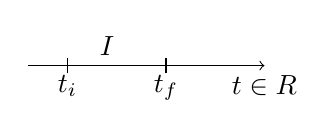
\begin{tikzpicture}
      \draw [->] (0,0) --++ (3,0) node [below] {$t \in \mathbbm R$};
      \node [below] at (.5,0) {$t_i$} node [below] at (1.75,0) {$t_f$}
       node [above] at (1,0) {$I$};
      \draw (.5,-.1) --++ (0,.2) (1.75,-.1) --++ (0,.2);
    \end{tikzpicture}
  \end{minipage}
  \hspace*\fill
  \textrightarrow The space $M$ \textleftarrow
  \hspace*\fill
  \begin{minipage}{.32\linewidth}
    \centering
    \begin{tikzpicture}
      \draw [->] (-.5,0) -- (2,0) node [below] {$t$};
      \draw [->] (0,-.5) -- (0,2);
      \node at (1,1) {$\mathbb C$} node at (.5,1.5) {$z$};
    \end{tikzpicture}
  \end{minipage}
\end{center}
\[
  \phi(t) \mapsto \phi(z) \phi(\tau)
\]
Map from a real axix to the target space,
map from the imaginary axis in the complex plane to the target space.
The property of the two maps really colse link together.

In summary: First, from $t$ to $z$, $t \mapsto z$,
then choose Z to be part of the imaginary axis or numbers, i.e., $z = -\iu\tau$. As the following examples
\begin{framed}
  \begin{multicols}{3}
  \begin{example}
    $t \mapsto z = -\iu\tau$
  \end{example}
  \begin{example}
    $\d t \mapsto -\iu\d\tau$
  \end{example}
  \begin{example}
    $\pdv*{}t \mapsto \iu \pdv*{}\tau$
  \end{example}
  \begin{example}
    $\pdv*\phi t \equiv \dot \phi \mapsto \iu \dot\phi_\tau$
  \end{example}
  \begin{example}
    $\dot\phi^2 \mapsto -\dot\phi_\tau^2$
  \end{example}
  \end{multicols}
  \begin{example}[The Lagrangian]
    \[
      \mathcal L(\phi, \dot\phi)
    = \frac12m\dot\phi^2 - V(\phi)
      \mapsto -\frac12m\dot\phi_\tau^2 - V(\phi_\tau)
    = -\mathcal L_E(\phi_\tau, \dot \phi_\tau)
    \]
    where $E$ stands for Euclidean, contrast with Minkovsky,
    the distance in space-time
    \[
      \d s^2 = -\d t^2 + (\d x^2 + \d y^2 + \d z^2)
    = \d x^2 + \d y^2 + \d z^2 + \d \tau^2
    \]
    By going from $t$ on the real axis to $\tau$ on the imaginary axis, which is so-called the Wick Rotation.
  \end{example}
  \begin{example}[The Action]
    \[
      \iu S[\phi] \equiv (\iu ) \int_{t_1}^{t_f} \d t \mathcal L
    \mapsto - S_E[\phi_\tau]
    \]
    where
    \[
      S_E[\phi_\tau] = \int_{\tau_i}^{\tau_f} \d\tau \mathcal L_E
    \]
  \end{example}
\end{framed}
So, after the integral, the propagator should be
\[
  \int_{x(t_{i,f}) = x_{i,f}} \mathcal D x(t) \upe^{\iu S[x(t)]} \mapsto
  \int \mathcal D x(\tau) \upe^{-S_E[x(\tau)]},\qq{where}
  \mathcal D \sim \sum_{x(\tau)}
\]
In \textbf{\textsf{Example 2.2.7}}, if we use $x$ as the new variable, i.e., $\phi \to x_i$
\[
  \mathcal L(\phi, \dot\phi) = \frac12 m\dot x^2 - V(x)
  \longrightarrow
  \mathcal L_E(x_\tau, \dot x_\tau) = \frac12 m\dot x_\tau^2 + V(x_\tau)
\]
The string can be displace in one direction. On the top of the string of each $\tau$, we change from $\dot x_t^2 \sim [x(\tau_n) - x(\tau_{n-1})]^2$
\begin{center}
  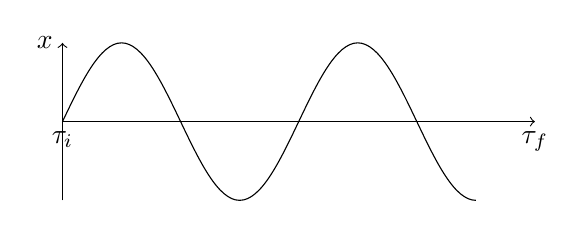
\begin{tikzpicture}
    \draw [->] (0,0) node [below] {$\tau_i$} --++ (6,0) node [below] {$\tau_f$};
    \draw [->] (0,-1) -- (0,1) node [left] {$x$};
    \draw (0,0) sin (.75,1) cos (1.5,0) sin (2.25,-1) cos (3,0)
                sin (3.75,1) cos (4.5,0) sin (5.25,-1);
  \end{tikzpicture}
\end{center}
We can interrupt it with tension $x(\tau)$ and potention $V(x(\tau))$,
completely a classical problem.
So, in the end, $\mathcal L_E$ is the energy density respects to the $\tau$-axis after the translation.
Concerning $S_E$
\[
  S_E[x(\tau)] = \int \d\tau \mathcal L_E(x(t), \dot x(t))
\]
it is of course the total energy after the translation.
In other words, $t$ is replaced by $\tau$.
i.e., in $\mathbb R^{d+1}$,
$d$ is supposed to the space dimension, and one for time.

\subsection{Quantum P.F.}

The partition function is
\begin{equation}
  Z = \Tr \upe^{-\beta\hat H}, \qq{where} \hat H = \frac{\hat p^2}{2m} + V(\hat x)
\end{equation}
where trace can be identity, i.e.,
\[
  Z_n = \int \d x_n \braket<x_0|\upe^{-\beta\hat H}|x_0>
\]
by inserting the identity $\int \d x_0 \ketbra|x_0><x_0| = \identity$.
What we need to do is to compare
\[
  \braket<x_0|\upe^{-\beta\hat H}|x_0> \qq{with}
  \braket<x_f|\hat U(t_f, t_i)|x_i>
\]
by slicing $\beta \sim t_f - t_i$ into $N$ pieces, each segment has a length of
$\delta \tau = \beta/N$. Then
\[
  Z = \int \d x_0 \d x_1 \cdots \d x_{N-1}
      \braket<x_0|\upe^{-\delta\tau\hat H}|x_{N-1}> \cdots
      \braket<x_n|\upe^{-\delta\tau\hat H}|x_{n-1}> \cdots
      \braket<x_1|\upe^{-\delta\tau\hat H}|x_0>
\]
What we have derived is
\[
  \braket<x_n|\upe^{-\frac\iu\hbar\delta t\hat H}|x_{n-1}>
= \ab(\frac{m}{2\pi\iu\hbar\delta t})^{1/2} \upe^{-\frac\iu\hbar \mathcal L(x_n, \dot x_n)\delta t}
\]
simply replace $\frac\iu\hbar\delta t \to \delta \tau$, then
\[
  \braket<x_n|\upe^{-\delta\tau\hat H}|x_{n-1}>
= \ab(\frac m{2\pi\hbar\delta\tau})^{1/2} \upe^{-\mathcal L_E(x(\tau_n), \dot x(\tau_n))\delta\tau}
\]
with the periodic boundary condition $x_N \equiv x_0$,
substitute it back, the partition function becomes
\begin{equation}
  Z = \ab(\frac{m}{2\pi\iu\hbar\delta t})^{N/2} \int \prod_{n=0}^{N-1} \d x_n
  \upe^{-\sum_{n=0}^{N-1} \delta\tau \mathcal L_E(x(\tau_n), \dot x(\tau_n))}
  \xlongequal{N\to\infty} \int_{x(0) = x(f)} \mathcal D x(\tau) \upe^{-S_E[x(\tau)]}
\end{equation}
then the action
\begin{equation}
  S_E[x_\tau] = \int_{0}^\beta \d \tau \mathcal L_E(x(\tau), \dot x(\tau))
\end{equation}

\paragraph{Quiz}

\begin{problem}
  Gaussian Integral
  \[
    \int \d x_1 \d x_2 \upe^{-(x_1,x_2) \begin{psmallmatrix}
      1 & \sfrac12\\\sfrac12 & 1
    \end{psmallmatrix} \begin{psmallmatrix}
      x_1\\x_2
    \end{psmallmatrix}}
  \]
  \rule{\linewidth}{1pt}
  Change the variable $x$ to a vector $\bm x = (x_1, x_2)$, i.e.
  \[
    \int \d\bm x \upe^{-\bm x \cdot \mathbf A \cdot \bm x}
  = \det\ab(\frac{\mathbf A}{\pi})^{-1/2}
  \]
\end{problem}

\begin{problem}
  \[
    F[\pi] = \frac12 \int_{t_i}^{t_f} \d t_1 \d t_2 \phi(t_1) A(t_1,t_2) \phi(t_2)
  \]
  then compute the second derivative $(\delta_\phi^2F)[\eta]$.\\
  \rule{\linewidth}{1pt}
  \[
    (\delta_\phi^2F)[\eta] = 2F[\eta]
  \]
\end{problem}

\begin{problem}
  The Lagrangian
  \[
    L(\phi_t, \dot\phi_t) = a\phi_t^2 + b\dot\phi_t^2 + c\phi_t\dot\phi_t
  \]
  show that $S[\phi] = S[\phi_c] + S[\phi - \phi_c]$,
  where $\phi_c$ is a classical path: $(\delta_\phi S)\big|_{\phi=\phi_c} = 0$.\\
  \rule{\linewidth}{1pt}
  Taylo expansion to $S[x + \eta]$
  \[
    S[x_c + \eta] = S[x] + (\delta_{x_c} S[\eta]) + \frac12(\delta_{x_c}^2S)[\eta]
  = S[x_c] + 0 + S[\eta]
  \]
\end{problem}

\paragraph{Case study}

We start from a Lagrangian
\begin{equation}
  \mathcal L(x(t), \dot x(t)) = \frac12m\dot x^2 - \frac12m\omega^2 x^2
\end{equation}
and we want to compute the propagator
$\int_{x(t_{i,f}) = x_{i,f}} \mathcal D(x) \upe^{\iu S[x(t)]}$.
This computation would be purely quantum.
We choose the staring point: $x(t_{i,f}) = x_{i,f}$.
We separate
\[
  x(t) = x_c(t) + \eta(t)
\]
Since $x_i$ and $x_f$ are fixed, so we get the boundary condition $\eta(t_i) = \eta(t_f) = 0$. Then the action
\[
  S[x_c + \eta]
= \upe^{\iu S[x_c]} \cdot \int_{\eta(t_i) = \eta(t_f) = 0} \mathcal D\eta(t) \upe^{\iu S{[\eta(t)]}}
\]
where $S[x(t)] = S[x_c] + S[\eta_c]$.
\begin{enumext}
  \item Comput $S[x_c]$
  \[
    S[x_c] = \int_{t_i}^{t_f} \d t \mathcal L(x_c(t), \dot x_c(t))
  = \int_{t_i}^{t_f} \mathcal L(t)
  \]
  Concering $x_c(t)$, using the E-L eq. (EOM)
  \[
    \odv*{\pdv{\mathcal L}{\dot x}}t - \pdv{\mathcal L}x = 0, \qq{or}
    (\pdif t^2 + \omega^2) x(t) = 0
  \]
  Before getting the solution, applying the boundary condition
  \[
    x(t_i) = x_i, \qq{and} x(t_f) = x_f
  \]
  The solution would be generally
  \[
    x_c(t) = x_0 \sin(\omega t + \phi_0)
  \]
  where $x_0$ and $\phi_0$ will be fixed by the boundary condition.
  Substitute it into the Lagrangian
  \[
    \mathcal L_{x_c}(t) = \frac12 m\omega^2 x0^2 \cos[2(\omega t + \phi_0)]
  \]
  and the actioin
  \[
    S[x_c] = \frac{m\omega}{2\sin(\omega\Delta t)}
             [(x_i^2 + x_f^2) \cos(\omega\Delta t) - 2x_ix_f]
  \]
  Now, we shall handle
  \[
    \int \mathcal D\eta \upe^{\iu S[\eta]}, \qq{where}
    S[\eta] = \int_{t_i}^{t_f} \d t
              \ab(\frac12 m\dot\eta^2 - \frac12 m\omega^2\eta^2)
  \]
  Referring \textbf{\textsf{Quiz 0.9}},
  $\int \d\bm x \upe^{-\bm x \cdot \mathbf A \bm x}$, we can convert the integral kernel to
  \[
    -\frac12 m\eta (\pdif t^2 + \omega^2) \eta
  \]
  where $(\pdif t^2 + \omega^2)$ is the ``sandwich'' term $\mathbf A$.
  Since
  \[
    \int \d t \dot\eta^2 = \cancel{(\eta\dot\eta)\big|_{t_i}^{t_f}}
  - \int \d t \ddot\eta
  \]
  Then the expression of the action is
  \[
    \int \mathcal D \eta \upe^{\iu S[\eta]}
  = \det\ab(\frac{\mathbf A}{\pi})^{-1/2}
  = \det\ab[\frac{\iu m}{2\pi}(\pdif t^2 + \omega^2)]^{-1/2}
  \]
  Given a matrix $M$, its determent $\det(\mathbf M) = \prod_i \lambda_i$,
  where $\lambda_i$ is the eigenvalue of $\mathbf M$. That is how we interrupt the determine of $\mathbf A$
  \[
    (\pdif t^2 + \omega^2)\psi_n = \lambda_n \psi_n
  \]
  We just define $X$
  \[
    X = \det(\pdif t^2 + \omega^2)
  = \prod_n \lambda_n 
  \]
  we need to solve the ODE by applying the boundary condition $\eta(t_i) = \eta(t_f) = 0$, i.e., $\psi_n(t_i) = \psi_n(t_f) = 0$.
  The eigenvalue
  \[
    \lambda_n = \omega^2 - (n\pi/\Delta t)^2
  = \omega^2- (n\Omega)^2, \quad n = 1, 2, \ldots, \infty
  \]
  and substitute it into $X$
  \[
    X = \prod_n \ab(\omega^2 - n^2\Omega^2)
  \]
  Take the log
  \[
    \ln X = \sum_n \ln(\omega^2 - n^2 \Omega^2)
  \]
  then take the derivative of $\omega$
  \[
    \pdv{\ln X}\omega = \sum_{n=1}^\infty \frac{2\omega}{\omega^2 - n^2\Omega^2}
  = \frac\pi\Omega \cotan \ab(\frac{\pi\omega}{\Omega}) - \frac1\omega
  \]
  integral to both sides
  \[
    \ln X = \ln\ab(\frac{\sin \omega\Delta t}{\omega} + \text{Const})
  \]
  Directly jump to the determine
  \[
    \det(\quad)^{-1/2} = C\ab(\frac{\omega}{\sim(\omega\Delta t)})^{1/2}
  \]
  When $\omega \to 0$, the Lagrangian
  \[
    \mathcal L = \frac12 m\dot x^2
  \]
  which is the free particle, and the determine $\det(\quad)^{-1/2} \sim \Delta t^{-1/2}$.
  For the boundaty condition of the free particle
  \[
    \braket<x=0|\upe^{-\frac\iu\hbar\hat H_0\Delta t}|x=0>
  = \int \d x \braket<x = 0|k> \upe^{-\iu\frac{\hat k^2}{2m} \Delta t}
    \braket<k|x = 0>
  = \frac1{2\pi} \int \d k \upe^{-\iu\frac{k^2}{2m}\Delta t}
  = \ab(\frac{m}{2\pi\iu\Delta t})^{1/2}
  \]
  where $H_0 = \frac{\hat p^2}{2m} = \frac{\hat k^2}{2m}$, set $\hbar = 1$,
  and $\braket<x|k> = \frac1{\sqrt{2\pi}} \upe^{\iu kx}$.
  To infer $C$, comparing the result with the determine
  \[
    \ab(\frac{m}{2\pi\iu\Delta t})^{1/2} = (\Delta)^{-1/2}, \qq{and}
    C = \ab(\frac m{2\pi\iu})^{1/2}
  \]
  Then we get $X$.
  \[
    \psi_n(t) \sim \sin \ab[\frac{n\pi}{\Delta t}(t - t_i)]
  \]
  Then substitute it into the ODE to obtain the normalization constant.
\end{enumext}

\section{PI \& Correlation functions}

Review what we get in the last section
\begin{equation}
  \begin{aligned}
    Z & = \int \d x_0 \upe^{\underset{x_i = x_f = x_0}{\iu S[x_c]}} \ab[\frac{m\omega}{2\pi\iu\sin(\omega t)}]^{1/2}\\
  & = \ab[\frac\pi{\iu m\omega \tan(\omega\Delta t/2)} \cdot
      \frac{m\omega}{2\pi\iu\sin(\Omega\Delta t)}]^{1/2}
    \xlongequal{\Delta \mapsto -\iu\beta}
      \ab[2\sinh\ab(\frac{\beta\omega}{2})]^{-1}
  \end{aligned}
\end{equation}
where the action
\begin{equation}
  S[x_c] = \frac{m\omega}{2\sin\omega\Delta t}
            [(x_i^2 + x_f^2) \cos(\omega\Delta t) - 2x_ix_f]
  \xlongequal{x_i=x_f=x_0} -\ab(m\omega \tan\frac{\omega\Delta t}{2}) x_0^2
\end{equation}
Two key points we need to keep in mind
\begin{itemize}
  \item The time interval $\Delta t \equiv t_f - t_i$,
  from the dictionary (Wick rotation) $t \mapsto -\iu\tau$,
  then $\Delta t \mapsto -\iu\beta$.
  \item The periodic boundary condition $x_i = x_f = x_0$.
\end{itemize}
The partition function should be like
\begin{equation}
  Z = \Tr\ab[\upe^{-\beta\omega\ab(\hat n+\frac12)}]
= \sum_{n=0}^\infty \upe^{-\beta\omega\ab(n+\frac12)}
= \frac{\upe^{-\beta\omega/2}}{1 - \upe^{-\beta\omega}}
  \equiv \ab[2\sinh\ab(\frac{\beta\omega}{2})]^{-1}
\end{equation}
where we have two context
\begin{enumext}
  \item Quantum mechaincs context $\braket<x_f|\hat U(t_f, t_i)|x_i>$
  \item Statistics mechanics context
\end{enumext}
\hrule
The path integration
\[
  \frac ZZ = \sum_{\underset{\text{configuration}}{\phi}} \frac{\rho[\phi]}{Z}
\]
where $\rho$ is so-called the raw probability, and $\rho[\phi]/Z$ is the actual probability.
Distinguish $\upe^{\iu S}$, $\upe^{-S_E}$, $\upe^{\beta H}$.
\begin{center}
  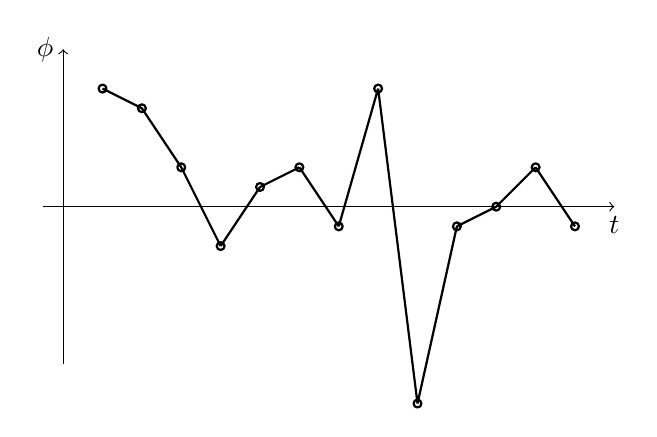
\begin{tikzpicture}[xscale = .5]
    \draw [->] (-.5,0) -- (14,0) node [below] {$t$};
    \draw [->] (0,-2) -- (0,2) node [left] {$\phi$};
    \draw [thick, rounded corners = .5cm, line join = round]
      (1,1.5) ellipse (.1 and .05) -- (2,1.25) ellipse (.1 and .05) --
      (3,.5)  ellipse (.1 and .05) -- (4,-.5)  ellipse (.1 and .05) --
      (5,.25)  ellipse (.1 and .05) -- (6,.5)  ellipse (.1 and .05) --
      (7,-.25) ellipse (.1 and .05) -- (8,1.5) ellipse (.1 and .05) --
      (9,-2.5) ellipse (.1 and .05) -- (10,-.25) ellipse (.1 and .05) --
      (11,0)   ellipse (.1 and .05) -- (12,.5) ellipse (.1 and .05) --
      (13,-.25) ellipse (.1 and .05);
  \end{tikzpicture}
\end{center}
If one measure for many tims, he may get something like a curve.
\[
  \frac1N \sum_i \phi_i \xlongequal{N\to\infty} \braket<\phi>
= \int \d\phi(\phi)\phi
\]
and
\[
  \frac1N \sum_i \phi_i = \braket<\phi^2> = \int \d\phi p(\phi)\phi^2z \phi^2
\]
and we call $\braket<\hat \phi>$, $n$-th moments. The variance
\[
  (\phi - \braket<\phi>)^2 = \braket<\phi>^2 - \braket<\phi^2>
\]
Caldular $\phi$
\begin{align}
  \braket<\phi^2>^d = \braket<\phi - \phi>^3, \qq{cumulants}
  \braket<\phi>^3 = \braket<\phi^3> - \braket<\phi>^3
\end{align}
Computing $\braket<\phi_i, \phi_j>$, where $i$ and $j$ can be treated as
different time. We define
\begin{equation}
  \frac1{N_\phi}\sum_{\phi(t)} \phi_i \phi_j = \braket<\phi_i \phi_j>
= \int\mathcal D\phi p[\phi] \cdot \phi_i \phi_j
\end{equation}
$N_\phi$ means how many times we take the sequence.
Means integrating with all the configurations. This is the correlation function we are talking about.

What we care about more is $\frac1N \sum_i \phi_i \phi_{i+\delta}$ instead the specific $i$ and $j$.

We can also expand to
\[
  \braket<\phi_i\phi_j\cdots\phi_n>
= \braket<\phi_i\phi_j\cdots\phi_n> -
  (a\braket<\phi_i>\braket<\phi_i\phi_j\cdots\phi_n>
+ b\braket<\phi_i\phi_j>\braket<\phi_i\phi_j\cdots\phi_n> + \cdots +
  c\braket<\phi_i> \braket<\phi_j> \cdots \braket<\phi_n>)
\]

\subsection{Generating Function(al) SI Partition Function}

\paragraph{Generating Function}

The set
\[
  \{m_0, m_1, m_2, m_3, \cdots\}
\]
We introduce a function of auxiliary variable $a$
\begin{equation}
  f(a) = m_0 + m_1a + \frac12m_2a^2 + \frac1{3!} m_3a^3 + \cdots
= \sum_{n=0}^\infty \frac1{n!} m_n a^n
\end{equation}
We just let the set of numbers as the series coefficients. In the end, we have
\[
  C_n = \odv[n]fa \bigg|_{a=0}
\]
and we treat $m_n$ as
\begin{equation}
  m_n = \braket<\phi^n> = \int\d\phi p(\phi) \phi^n
\end{equation}
Then, $f(a)$ becomes
\begin{equation}
  f_m(a) = \sum_n \frac1{n!} a^n \int \d\phi p(\phi)\phi^n
= \int\d\phi p(\phi) \upe^{a\phi} = \braket<\upe^{a\phi}>, \quad
  f_c(a) = \ln f_m(a)
\end{equation}
where $m_0 = 1$.
\begin{align*}
  K_0 & = f_c(0) = \ln f_m(0) = \ln m_0 = 0,\\
  K_1 & = \odv{f_C(a)}a \bigg|_{a=0}
= \frac1{f_m(0)} \odv{f_m(a)}a \bigg|_{a=0} = m_1,\\
  K_2 & = \odv[2]{f_C(a)}a\bigg|_{a=0} = \frac{f''_m(a) f_m(a) - f'_m(a) f_m'(a)}{f_m^2(a)}\bigg|_{a=0}
= m_2 - m_1^2 = \braket<\phi^2> - \braket<\phi>^2\\
  K_3 & = \odv*[fun]{\frac{f_m'}{f_m} - \ab(\frac{f_m'}{f_m})^2}a
= \frac{f_m^{(3)}f_m - f_m''f_m'}{f_m^2} - 2\frac{f_m'}{f_m} \frac{f_m''f_m - f_m'f_m'}{f_m^2}\bigg|_{a=0}\\
& = m_3 - 3m_2m_1 + 2m_1^3 = \braket<\phi^3> - 3\braket<\phi^2>\braket<\phi> + 2\braket<\phi>^3
\end{align*}

\paragraph{Generating Function\textcolor{red}{al}}

\begin{center}
  \begin{tabular}{llll}
    \toprule
    Function    & $f(\phi)$    & single variable             & $\phi$\\
    Functional  & $F[\phi(t)]$ & multiple variable / vector  & $\{\phi_i\}$\\
                &           & continous variables         & $\phi(t)$ (function)\\
    \bottomrule
  \end{tabular}
\end{center}

Now the coefficients set becomes
\[
  \{C_0,\ C_1(x),\ C_2(x_1,x_2),\ \ldots\,,~C_n(x_1,\ x_2,\ \ldots\,,~x_n),\ \ldots\}
\]
Then the auxiliary function is $a(x)$
\begin{multline}
  F[a(x)] = C_0 + \int \d x_1 C_1(x_1) a(x_1)
      + \frac1{2!} \int\d x_1\d x_2 C_2(x_1x_2) a(x_1)a(x_2) + \cdots\\
      + \frac1{n!} \int \d x_1 \cdots \d x_n C_n(x_1,\ x_2,\ \ldots\,,~x_n)
        a(x_1) a(x_2) \cdots a(x_n)
\end{multline}
Each term here to the $n$-th order is we used to call the functional derivative $(\delta^nF)[a]$.
Considering $C_n$
\[
  C_n(x_1,\ x_2,\ \ldots\,,~x_n) \sim
  \braket<\phi(x_1) \phi(x_2) \cdots \phi(x_n)>
= \fdv{F^n[a]}{a(x_1), a(x_2), \cdots, a(x_n)}\bigg|_{a=0}
\]
\begin{framed}
  Someone hasn't understand functional (derivative) NOW!!!

  $a = (a_1, a_2)$, $\phi = (\phi_1, \phi_1)$.
  \[
    F[a] = a_1\phi_1 + a_2\phi_2 = \sum_{i=1}^2 a_i\phi_i = a^{\mathsf T}\phi
  \]
  \[
    C_{i=1,2}^{(1)} = \fdv F{a_{1,2}} = \phi_{1,2}, \quad
    C_{ij}^{(2)} = \fdv[2]F{a_i,a_j},
  \]
  or more complex
  \[
    F[a] = (a_1, a_2) \mathbf A_{2\times 2} \begin{pmatrix}
      a_1\\a_2
    \end{pmatrix} = a^{\mathsf T}\mathbf A a
  \]
\end{framed}

\paragraph{Quiz}
\begin{example}
  \[
    C_n(x_1,\ x_2,\ \ldots\,,~x_n) = \braket<\phi(x_1) \phi(x_2) \cdots \phi(x_n)>
  = \int \mathcal D\phi p[\phi] \phi(x_1) \phi(x_2) \cdots \phi(x_n)
  \]
  Calculate the generating function $F[a(x)]$ first.
  \[
    F[a(x)] = \int \mathcal D\phi p[\phi] \upe^{\int \d x a(x) p(x)}
  = \braket*\big<\upe^{a^{\mathsf T}\phi}>
  \]
  Consider $p[\phi]/Z$, $Z = \int\mathcal D\phi p[\phi]$,
  where $p[\phi] = \upe^{-S_E[p]}$.
  Write $F[a(x)]$ explicitly
  \[
    F[a(x)] \xlongequal{p[\phi]=\upe^{-S[\phi]}/Z} \frac1Z
    \underbrace{\int \mathcal D\phi \upe^{-\frac{S[\phi]-a^{\mathsf T}\phi}{S_a[\phi]}}}_{Z_a}
  = \frac{Z_a}{Z_0}
  \]
  where $a$ is the \emph{control variable},
  and $\phi$ is the \emph{system variable}.
  $Z_a$ can be $Z_a(\mathbf H, \mathbf m)$ or $Z_a(\mathbf A, \mathbf j)$.
  \[
    \pdv{\braket<m(x_1)>}{h(x_2)}\bigg|_{h=0}
  = \fdv*[fun]{\fdv{F[h]}{h(x_1)}}{h(x_2)} = \braket<m(x_1) m(x_2)>|_{h=0}
  \]
  In contrast, $h$ is $a$, $m$ is $\phi$. It's what we called the \emph{susceptibility}, or \emph{linear response function}.
\end{example}

\begin{example}
  Action function $S[\phi] = \frac12 \phi^{\mathsf T} A\phi$.
  Calculate $\braket<\phi_i, \phi_j>$.
  \[
    Z_a = \int \mathcal D\phi \upe^{-S[\phi]+a^{\mathsf T}\phi}
  = \int\mathcal D\phi \upe^{-\frac12\phi^{\mathsf T}A\phi + a^{\mathsf T\phi}}
  = \det\ab(2\pi\mathbf A^{-1})^{1/2} \upe^{a^{\mathsf T}\mathbf A^{-1}a/2},
    \quad
    Z_0 = Z_a\big|_{a=0}.
  \]
  and $Z_0$ is just the Gaussian term.
  \[  
  F[a] = \frac{Z_a}{Z_0} = \upe^{a^{\mathsf T}\mathbf A^{-1}a/2}
  \]
  Define $\mathbf A^{-1} = G$, matsubara Green function.
  \[
    \braket<\phi_i\phi_j> = \pdv F{a_i, a_j}\bigg|_{a=0}
  = G_{ij}
  \]
\end{example}

\paragraph{Quiz 8}

Make a sentense with the following phrases:

\textbf{Path Integral}
\textbf{Partition Function} (is)
\textbf{Generating Functional} (of)
\textbf{Correlation Functions}

and combine them with ``is'', ``are'', ``of'', ``at'', ``on'', ``in'', ``below'', ``above'', etc.

DeepSeek: The Path Integral formulation of quantum mechanics reveals that the Partition Function is a specific type of Generating Functional, from which all Correlation Functions can be derived by taking functional derivatives."

\paragraph{Explanation}

The partition function
\[
  Z = \sum_n \upe^{-\beta E_n}
\]
is a kind of generating function, i.e., we want the average and the fluctuation of energy
\[
  \braket<E>, \qq{and} \braket<E^2> - \braket<E>^2
\]
So, the Generating function for energy is, for momentum, we try to evalute
\[
  f_m(a) = \braket<\upe^{aE}> = \frac1{Z_0} \underbrace{\sum_n \upe^{(a-\beta) E_n}}_{Z_a} = \frac{Z_a}{Z_0}
\]
Then, the critical generating function
\[
  f_c = \ln f_m(a) = \ln Z_a - \ln Z_0
\]
Since $\braket<E^2>^c = \braket<E^2> - \braket<E>^2$, then the cumulent
\[
  \braket<E>^c = \braket<E> = \odv*{f_c(a)}a \bigg|_{a=0}
= \odv{\ln Z}a \bigg|_{a=0} = -\odv{\ln Z}\beta
\]
By construction, the cumulent
\[
  \braket<E^2>^c = \braket<E^2> - \braket<E>^2 = \odv[2]{f_C(a)}a\bigg|_{a=0}
= \odv[2]{\ln Z}\beta
\equiv \frac{\beta^2}{k_B}C_v
\]
\rule \linewidth {.5pt}
In the new context, upgrade to ``functional'': consider the general form of the
partition function
\[
  \mathcal Z = \int \mathcal D\phi(\tau) \upe^{-\mathcal S_E[\phi]}
\]
we integrate over all the configuration, since they are very complicated, so we
use the ``fancy'' expression.

Starting from the $n$-point correlation function
\[
  \braket<\phi(\tau_1) \phi(\tau_2) \cdots \phi(\tau_n)>
  \xlongequal{\text{variables are continous}}
  \braket<\phi_i \phi_j \cdots \phi_l>^{(c)} =
  \pdv[n-3]{F_{m,c}[a]}{a_i, a_j, \cdots, a_l} \bigg|_{a=0}
\]
and the definition of $F_m[a]$ is
\[
  F_m[a] = \braket<e^{a\tran\phi}>
= \frac1Z \int \mathcal D\phi
  \upe^{-S_E + \underset{\text{`source' term}}{\underline{a\tran\phi}}}
= \frac{Z_a}{Z_0}
\]
where we take $Z_a = \upe^{-S_a}$ and $S_a = S_E - a\tran\phi$.
The term $a\tran\phi = \phi\tran a$ is symmetric, can be expressed as
\[
  a\tran\phi = \int \d\tau a(\tau) \phi(\tau) \sim \sum_i a_i \phi_i
\]
and critical one is $F_c[a] \sim \ln Z_a$.

Then the fluctuation
\[
  \braket<\phi_i\phi_j>^c
= \braket<\phi_i\phi_j> - \braket<\phi_i>\braket<\phi_j>.
\]
Define
\[
  (\chi_\phi)_{ij} = \pdv{\braket<\phi_i>_a}{a_j}\bigg|_{a=0}
= \pdv*{\pdv{F_c[a]}{a_i}}{a_j} \bigg|_{a=0}
= \pdv{\ln Z_a}{a_i a_j} \bigg|_{a=0} \equiv \braket<\phi_i\phi_j>^c
\]
This relation, is so-called the \emph{Fluctuation-Dissipation Theorem}.

\section{Green's Function}

Consider
\[
  S_{E, \text{or} a}[\phi] = \frac12 \phi\tran A\phi - a\tran\phi
\]
which is the same format of $S_a = S_0 - a\tran\phi$, and $A$ is symmetric,
$A = A\tran$.
Here,
\[
  \phi\tran A\phi = \sum_{ij} A_{ij} \phi_i \phi_j
= \int \d\tau \d\tau' A(\tau, \tau') \phi(\tau) \phi(\tau')
\]
$A$ is symmetric. Then,
\[
  F_m[a] = \frac{Z_a}{Z_0}
= \frac{\int\mathcal D\phi \upe^{-S_a}}{\int \mathcal D\phi \upe^{-S_0}}
= \upe^{\frac12 a\tran A^{-1} a}
\]
we define the Green's function is the inverse
\begin{equation}
  G \equiv A^{-1}, \qq{or} AG = \identity
\end{equation}
Rewrite it
\[
  \sum_j A_{ij} G_{jl} = \delta_{il}
\]
make it continuous
\[
  \int \d\tau A(\tau_1, \tau) G(\tau, \tau_2) = \delta(\tau_1 - \tau_2)
\]
The propagator $\braket<x_f|\hat U(t_f,t_i)|x_i>$ can be just what Green's
function is. The EOM here can be
\[
  \delta\phi S_a = 0
\]
\begin{enumext}
  \item then we have
  \[
    \delta\phi S_a[\eta]
  = \odv{S[\phi + \epsilon\eta]}\epsilon\bigg|_{\epsilon=0}
  = \frac12(\eta\tran A\phi + \phi\tran A\eta) - a\tran\eta
  \xlongequal[a\tran\eta=\eta\tran a]{\phi\tran A\eta = \eta\tran A\phi}
    \eta\tran(A\phi - a)
  \]
  The solution is
  \[
    A\phi = a, \qq{exist} A\phi_0, \qq{then}
    \phi_c = A^{-1}a + \phi_0 \xlongequal{G\equiv A^{-1}} Ga + \phi_0
  \]
  where $G$ can be a matrix, $a$ can be a vector. Now, $\phi_c(\tau)$ can be
  \[
    \phi_c(\tau) = \int \d\tau'
    \underset{\text{propagator}}{\underline{G(\tau, \tau')}} \,
    \underset{\text{source}}{\underline{a(\tau')}} + \phi_0(\tau)
  \]
  the source $a(\tau)$ can be charge distribution,
  $\phi$ can be the field propagated by the charge.
  \item The functional derivative
  \[
    \fdv{S_a[\phi]}{\phi_i} = \sum_j A_{ij} \phi_j - a_i = 0
  \]
  since $\sum_{jl} A_{jl} \phi_j \phi_l = \phi\tran A\phi$ and
  $a\tran\phi = \sum_j a_j\phi_j$.
\end{enumext}

\paragraph{Case study: Quantum Harmonic Oscillator}

The Hamiltonian ($\hbar = 0$)
\[
  \hat H = \frac{\hat k^2}{2m} + \frac12m\omega^2\hat x^2
\]
which is basically the Canonical Quantization.
Then, we can write down the Path Integral form. We need the Lagrangian
\[
  \mathcal L(x(t), \dot x(t)) = \frac12 m(\dot x^2 - \omega^2x^2)
\]
The action is a functional of
\[
  \mathcal S[x(t)] = \int_{t_i}^{t_f} \d t \mathcal L(x, \dot x)
= -\int_{t_i}^{t_f} \d t \frac12mx(t) (\pdif t^2 + \omega^2) x(t)
  +S_\text{boundary term}
\]
The $S_\text{boundary term}$ is due to ``integral by part''.
Therefore
\[
  \mathcal Z = \int \mathcal D x\upe^{\iu\mathcal S[x]}
\]
one can let $\iu t \leftrightarrow \tau$.
The Wick rotation version can be $\iu\mathcal S \leftrightarrow -S_E$,
and the Euclidian version can be
$S \leftrightarrow S_E = \int_0^\beta \d\tau \mathcal L_E(x(\tau), \dot x(\tau))$,
and the boundary term does not appear here.
\[
  S_E = \int_0^\beta \d\tau \mathcal L_E(x(\tau), \dot x(\tau))
= \int_0^\beta \d\tau \frac12 mx(\tau) (\omega^2 - \pdif\tau^2) x(\tau)
\]
$\phi(\tau)$ is now replaced by $x(\tau)$, i.e.,
\[
  \frac12 x\tran A x = \frac12 \int_0^\beta \d\tau \int_0^\beta\d\tau'
  x(\tau) A(\tau,\tau') x(\tau')
\]
If we insert the identity $\int_0^\beta\d\tau' \delta(\tau - \tau')$,
then, we will have a prime for the first $x$, i.e.,
\[
  S_E = \int_0^\beta \d\tau \int_0^\beta \d\tau' \delta(\tau - \tau')
        \frac12 mx(\tau) (\omega^2 - \pdif\tau^2) x(\tau)
\]
Therefore, $A$ will be
\[
  A(\tau', \tau) = m\delta(\tau' - \tau) (\omega^2 - \pdif\tau^2)
\]
So, finally, we can use
\begin{equation}
  \int \d\tau A(\tau_1, \tau) G(\tau, \tau_2) = \delta(\tau_1 - \tau_2)
\end{equation}
to generate the Green's funciton.
\[
  \text{LHS} = \int \d\tau \delta(\tau_1 - \tau)
               [m(\omega^2 - \pdif \tau^2)] G(\tau, \tau_2)
= m(\omega^2 - \pdif{\tau_1}^2) G(\tau_1 - \tau_2)
= \delta(\tau_1 - \tau_2) = \text{RHS}
\]
Denote $\Delta\tau = \tau_1 - \tau_2$, then
\[
  \text{LHS} = m(\omega^2 - \pdif{\Delta_\tau}^2) G(\Delta\tau)
= \delta(\Delta\tau) = \text{RHS}
\]
and $G$ satisfies the periodic boundary condition
\[
  G(\Delta\tau) = G(\Delta\tau + \beta).
\]
means that if we have a range, $\tau \in [0, \beta]$,
and the fourier transform
\[
  \ab\{f_l(\tau) = \frac1{\sqrt\beta} \upe^{\iu\frac{2\pi}{\beta} l\tau}\}
\]
where $l \in \mathbb Z$ is a label.
Such that $G(\Delta\tau)$ can be expanded over this space
\begin{equation}
  G(\Delta\tau)
= \sum_l g_l \ab(\frac1{\sqrt\beta} \upe^{\iu\omega_l\Delta\tau})
\end{equation}
where we denote $\omega_l \equiv \frac{2\pi}{\beta}l$.
Then, the left hand side
\[
  \text{LHS} = \sum_l g_l m(\omega^2 + \omega_l^2)
  \ab(\frac1{\sqrt\beta} \upe^{\iu\omega_l \Delta\tau})
\]
Since the $\delta$-function, the right hand side
\[
  \text{RHS} = \delta(\Delta\tau)
= \sum_l \ab(\frac1{\sqrt\beta} \upe^{\iu\omega_l\Delta\tau}) \frac1{\sqrt\beta}
\]
which satisfies the orthogonality
\[
  \sum_l \ab(\frac1{\sqrt\beta} \upe^{\iu\omega_l\tau_2})^*
         \ab(\frac1{\sqrt\beta} \upe^{\iu\omega_l\tau_1})
= \sum_l \frac1\beta \upe^{\iu\omega_l\Delta\tau} = \delta(\Delta\tau)
\]
then, we will derive the coefficient
\[
  g_l = \frac1{\sqrt\beta} \frac{1}{m(\omega^2 + \omega_C^2)}
\]
Therefore, the Green's function, or the correlation function, is
\begin{equation}
  \braket<x(\tau_1) x(\tau_2)> =
  G(\Delta\tau) = \sum_l \frac1\beta
                  \frac{\upe^{\iu\omega_l\Delta\tau}}{m(\omega^2 + \omega_l^2)}
= \frac1{2\pi m} \int_{-\infty}^\infty \d\Omega
  \frac{\upe^{\iu\Omega\Delta t}}{\omega^2 + \Omega^2}
= \frac{\upe^{-\omega|\Delta\tau|}}{2\pi m}.
\end{equation}
where we denote $\omega \to \Omega$ when ground state $T\to0$, $\beta\to\infty$.
In order to obtain the compact form, consider when $\Delta\tau$ is larger/less
than zero, we need to use the Heavisine step function
\begin{equation}
  \braket<x(\tau_1) x(\tau_2)> = G(\Delta\tau)
= \theta(+\Delta\tau) \frac{\upe^{-\omega\Delta\tau}}{2m\omega}
+ \theta(-\Delta\tau) \frac{\upe^{\omega\Delta\tau}}{2m\omega}
\end{equation}
To do the Wick rotation, let $\Delta\tau \leftrightarrow \iu\Delta t$.
Then, $\theta(\Delta\tau) \leftrightarrow \theta(\Delta t)$,
$\iu G(\Delta\tau) \leftrightarrow G(\iu\Delta t)$, i.e., the
\emph{time-ordered Green's function} (in real time)
\begin{equation}
  G(\Delta t) = \theta(+\Delta t) \frac{\iu\upe^{-\iu\omega\Delta t}}{2m\omega}
              + \theta(-\Delta t) \frac{\iu\upe^{+\iu\omega\Delta t}}{2m\omega}
              = G^\text{ret}(\Delta t) + G^\text{adv}(\Delta t)
\end{equation}
and $\braket<x(\tau_1)x(\tau_2)> = \braket<x(\tau_2)x(\tau_1)>$.
To make it symmetric,
\begin{equation}
  \braket<\mathcal T \hat x(t_1) \hat x(t_2)>
= \underbrace{\theta(t_1 - t_2) \braket<\hat x(t_1) \hat x(t_2)>}_
  \text{operator definition of the Retarded Green functioin} +
  \underbrace{\theta(t_2 - t_1) \braket<\hat x(t_2) \hat x(t_1)>}_
  \text{operator definition of the Advanced Green functioin}
\end{equation}
where $\hat x(t) = \upe^{\iu\hat H t} \hat x\upe^{-\iu\hat H t}$.
To accurate it, consider the first term with respect to the ground state
\begin{align*}
    \iu\braket<0|\hat x(t_1) \hat x(t_2)|0>_{t_1>t_2} &
  = \iu\braket<0|
    \upe^{\iu\hat H t_1}\hat x \upe^{-\iu\hat H(t_1-t_2)}\hat x
    \upe^{-\iu\hat Ht_2}|0>
  = \iu \upe^{\iu(\frac12\omega)\Delta t}
    \braket<0|\hat x \upe^{-\iu\hat H\Delta t}\hat x|0>\\
& = \frac\iu{2m\omega} \upe^{\iu(\frac12\omega)\Delta t}
    \braket<1|\upe^{-\iu\hat H\Delta t}|1>
  = \frac\iu{2m\omega} \upe^{+\iu\ab(\frac12\omega)\Delta t}
                       \upe^{-\iu\ab(\frac32\omega)\Delta t}
\end{align*}
where $\hat H\ket|0> = \ab(\frac12\omega)\ket|0>$,
$\Delta t \equiv t_1 - t_2$, and
$\hat x = \frac1{\sqrt{2m\omega}}(\hat a + \hat a^\dagger)$.
Now, go back to the Formalism.

\noindent \rule \linewidth {1pt}

\paragraph{Wick Theorem}

Consider
\[
  \mathcal S[\phi] = \frac12\phi\tran A\phi
\]
and
\[
  \braket<\phi_i\phi_j \cdots\phi_l>
= \fdv[order = n-3, fun]{Z_a/Z_0}{a_i, a_j, ..., a_l}\bigg|_{a=0}
\]
apply Taylor-expansion to the factor
\[
  Z_a/Z_0 = \upe^{\frac12a\tran G a}
= 1 + \ab(\frac12a\tran Ga) + \frac1{2!}\ab(\frac12a\tran Ga)^2 + \cdots
+ \frac1{n!}\ab(\frac12a\tran Ga)^n + \cdots
\]
we denote $n$: $\underbrace{\braket<\phi_i\phi_j \cdots\phi_l>}_n$.
\begin{enumext}
  \item If $n$ is odd, then $\braket<\phi_i\phi_j \cdots\phi_l> = 0$.
  \item If $n$ is even, or let $n = 2n$,
  for any term contains the order of $a$ larger than the order of derivative,
  then this term will vanish since we take $a = 0$.
  Expand the secoond term
  \[
    (a\tran Ga)(a\tran Ga)
  = \ab(\sum_{i_1j_1} a_{i_1} G_{i_1j_1} a_{j_1})
    \ab(\sum_{i_2j_2} a_{i_2} G_{i_2j_2} a_{j_2})
  \]
  then
  \[
    \underbrace{\braket<\phi_i\phi_j \cdots \phi_l>}_{2n}
  = \sum_{(\quad)} (\quad) \underbrace{
    \overbrace{G_{i_1j_1}G_{i_2j_2}}^{\braket<\phi_{i_1}\phi_{j_1}>}
    \cdots G_{i_nj_n}}_n
  \]
  Let the labels $i\to\tau_1$, $j\to\tau_2$, \ldots, $l\to\tau_{2n}$.
  The map can be visualization as
  \begin{center}
    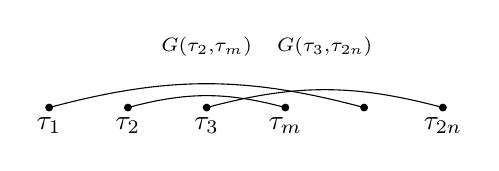
\begin{tikzpicture}
      \fill (1,0) circle (.05) node [below] {$\tau_1$};
      \fill (2,0) circle (.05) node [below] {$\tau_2$};
      \fill (3,0) circle (.05) node [below] {$\tau_3$};
      \fill (5,0) circle (.05);
      \fill (4,0) circle (.05) node [below] {$\tau_m$};
      \fill (6,0) circle (.05) node [below] {$\tau_{2n}$};
      \draw (1,0) to [bend left = 15] (5,0);
      \draw (2,0) to [bend left = 15] (4,0)
       node [above] at (3,15pt) {$\scriptstyle G(\tau_2, \tau_m)$};
      \draw (3,0) to [bend left = 15] (6,0)
       node [above] at (4.5,15pt) {$\scriptstyle G(\tau_3, \tau_{2n})$};
    \end{tikzpicture}
  \end{center}
  The accumulant version is
  \[
    \braket<\underbrace{\phi_i \cdots \phi_l}_n>^c
  = \fdv*[n]{\ab(\frac12a\tran Ga)}{a_i, ..., a_l}
  \]
\end{enumext}

\dbend
\begin{framed}
  Add the interaction term, i.e.,
  \[
    \mathcal S[\phi] = \frac12\phi\tran A\phi + \frac\lambda{4!} \phi^4
  \]
  $S_\text{int}$ is a functional of $\phi$
  \[
    S_\text{int} = \frac\lambda{4!} \phi^4 \sim
    \int \d\tau \phi^4(\tau)
  \]
  compare this guy maybe more general
  \[
    \int \d\tau_1 \d\tau_2 \d\tau_3 \d\tau_4
    A(\tau_1\tau_2\tau_3\tau_4)
    \phi(\tau_1) \phi(\tau_2) \phi(\tau_3) \phi(\tau_4)
  \]
  By Taylor expansion
  \[
    \upe^{-\sin t} = 1 + \frac\lambda{4!}\braket<\phi^4>
                   + \frac1{2!}\ab(\frac\lambda{4!}\braket<\phi^4>)^2 + \cdots
  \]
  Since $Z \to \int\mathcal D\phi\upe^{-S\Delta\tau}(\qquad)$
  and $Z_\text{int} \sim \braket<\upe^{-\sin t}>_0$,
  all the four point becomes
  \begin{align*}
    \begin{tikzpicture}[baseline = (a1.base)]
      \begin{feynhand}
        \vertex [dot] (a1) at (0,0) {};
        \vertex [dot] (b1) at (1,0) {};
        \vertex [dot] (c1) at (2,0) {};
        \vertex [dot] (d1) at (3,0) {};
        \propag       (a1) to [out = 90, in = 90] (b1);
        \propag       (c1) to [out = 90, in = 90] (d1);
      \end{feynhand}
    \end{tikzpicture}
    & \qq{$\longrightarrow$} 8\\
    \begin{tikzpicture}[baseline = (a2.base)]
      \begin{feynhand}
        \vertex [dot] (a2) at (0,0) {};
        \vertex [dot] (b2) at (1,0) {};
        \vertex [dot] (c2) at (2,0) {};
        \vertex [dot] (d2) at (3,0) {};
        \propag       (a2) to [out = 90, in = 90] (c2);
        \propag       (b2) to [out = 90, in = 90] (d2);
      \end{feynhand}
    \end{tikzpicture}
    & \qq{$\longrightarrow$} \infty\\
    \begin{tikzpicture}[baseline = (a3.base)]
      \begin{feynhand}
        \vertex [dot] (a3) at (0,0) {};
        \vertex [dot] (b3) at (1,0) {};
        \vertex [dot] (c3) at (2,0) {};
        \vertex [dot] (d3) at (3,0) {};
        \propag       (a3) to [out = 90, in = 90] (d3);
        \propag       (b3) to [out = 90, in = 90] (c3);
      \end{feynhand}
    \end{tikzpicture}
    & \qq{$\longrightarrow$} ?
  \end{align*}
  i.e., the core of Feynmann diagram.
\end{framed}
%  !TeX root = ../main.tex

\chapter{Symmetry}

\paragraph{What is symmetry?}

\begin{enumext}
  \item Leibniz: Symmetry is \emph{indiscernability of
    \sout{differences} changes \textrightarrow transformations}.
  \item Physical: invariance (under) transformations.
\end{enumext}

\subparagraph{Action part.}

V is the Hilbert space, and we have a map $V \mapsto V$, which is
the operator. The map is invertible.
Transformation stands for something like $X \mapsto \Omega(X)$,
i.e., map something to something else, but ``something else''
is in the same space, such as mapping a vector to a vector.
For example,
\[
\begin{cases*}
  \ket|\psi>  \mapsto \hat\Omega \ket|\psi>,& Transformation of state\\
  \hat O      \mapsto \hat\Omega \hat O \hat\Omega^{-1},
& Transformation of Operator\\
  \phi(x)     \mapsto (\Omega \phi)(x),     & Path Integral
\end{cases*}
\]

\subparagraph{Invariance part.}

When $X \sim Y$, i.e., $X$ is equivalent to $Y$, then it calles the
invariance.
After the map, we get something equivalent to $X$: $\Omega(x) \sim X$.
The invariance in the context can be, for example
\[
  \text{equations / constraints}\ \Omega(x) \sim X \longrightarrow
  \begin{cases*}
    \Omega \ket|\psi> = \ket|\psi> \upe^{\iu\varphi} &
    Transformation of state\\
    \hat\Omega \hat H \hat\Omega^{-1} = \hat H       &
    Transformation of Operator\\
    \mathcal S[\phi] = \mathcal S[\Omega\phi]        &
    Path Integral
  \end{cases*}
\]
To symmetry, $\Omega(x) \sim X$ is just equations/constraints:
Each equation is a kind of constraint on the object.

\vskip1ex \hrule
\subparagraph{Symmary}

For symmetry constraints, what constraints do is a limited possibility:
it is simplicity, or what understandability comes from.
How this happens is related to \emph{Symmetry \& Group Theory.}

The group is a set: we consider a set of transformation $\Omega_i$
\[
  G = \{\Omega_i\}, \qq{and the operation} \Omega_1 \circ \Omega_2
\]
The operation says that $\circ:\ G \times G \to G$.
Concerning the basic properties of Group
\begin{enumext}
  \item Closure: If $\Omega_{1,2}(X) \sim X$, then the combination
  $\Omega_1(\Omega_2(X)) \sim \Omega_i(X) \sim X$ is also in this set.
  \item Identity: Also okay, to do nothing.
  \item Inverse: We can have $\Omega(X) \sim X$ then do the inverse
  $\Omega^{-1}$ on both side
  \[
    X \sim \Omega^{-1}(X)
  \]
  By equivalent, this is so-called the inflective.
  \item Associativity: Such as by Hamiltonian, etc.
\end{enumext}
Referring to the Group theory, we shall talk about the

\section{Group Representation Theory}

\begin{enumext}
  \item Group: Introduce the space; elementary ``particles''
  \item Representation: We can ``lable'' (name) all the representations
  \begin{enumext}
    \item Different labels, which is closely related to conserved quantities
    (quantum numbers);
    \item Dimension: closely related to degeneracy.
  \end{enumext}
\end{enumext}

\subsection{Translation}

A trivial example is just to move the entire function $\phi(x)$ towards one
direction by $a$, we get
\[
  \phi(x) \mapsto \phi(x - a) \equiv \tilde \phi(x)
\]
where $x \in \mathbb R$. And we can define the translation operator $\hat T_a$
\[
  \phi(x - a) = \tilde \phi(x) = (\hat T_a\phi)(x)
\]
where $\phi(x)$ is the wavefunction, and we can get the new state
\[
  \phi(x) = \braket<x|\phi> \mapsto \phi(x - a) = \braket<x|\hat T_a\phi>
\]
Try to write it in the way of expansion
\[
  \hat T_a\ket|\phi> = \int \d x \ket|x> \braket<x|\hat T_a\phi>
= \int \d x \ket|x> \phi(x - a)
\xlongequal{\tilde x = x - a} \int \d x \ket|x - a> \phi(x)
\]
So, this transformation operator is a linear operator.
Insert the identity
\[
  \ket|\phi> = \int \d x \ket|x> \braket<x|\phi>, \qq{then,}
  \hat T_a\ket|\phi> = \int \d x \hat T_a \ket|x> \phi(x)
\]
In short, we have
\[
  \hat T_a\ket|x> = \ket|x + a>
\]
If $\ket|x>$ refers to a delta function $\delta(x)$, then the transformation
just move it to $\delta(x + a)$.
To write $T_a$ in basis
\[
  \hat T_a = \int \d x \ketbra|x + a><x|
\]
\paragraph{Quiz.}
Try to compute $\hat T_a \hat T_b$.
\[
  \hat T_a \hat T_b = \hat T_{a+b=b_a} = \hat T_b \hat T_a
\]

\subsection{Reflection}

\[
  \phi(x) \mapsto \phi(2a - x)
\]
We call the operation $\rho_a$.
The same logic.
\[
  \hat\rho_a\ket|\phi> = \int \d x \ket|x> \braket<x|\hat\rho_a\phi>
= \int \d x \ket|x> \phi(2a - x) = \int \d x \ket|2a - x> \phi(x)
\]
\textbf{Remember no minus sign here: the integration range also reversed.}
So, we obtain
\[
  \hat \rho_a\ket|x> = \ket|2a - x>
\]
\paragraph{Quiz}
Compute $\hat \rho_a \hat \rho_b$.
\[
  \hat\rho_a \hat\rho_b = \hat T_{2a - ab}
\]

\paragraph{Quiz}
Compute $\hat \rho_a \hat \rho_b \hat \rho_c$.
\[
  \hat\rho_a \hat\rho_b \hat\rho_c = \hat \rho_{a-b+c}
\]
There are some identities
\begin{align}
  \hat\rho_a^2 & = \identity,\\
  \hat\rho_a \hat\rho_b & \neq \hat\rho_b \hat\rho_a, \qq{where $a \neq b$}
\end{align}

\paragraph{Quiz}
Prove if $\hat T_a \hat \rho_b \overset?= \hat\rho_b\hat T_a$.
\[
  \hat T_a = \rho_{a/2} \rho_0
\]
So, $\hat T_a \hat \rho_b = \rho_{a/2+b}$, and
$\hat\rho_b\hat T_a = \rho_{b-a/2}$. They are not equal.

\subsection{Invariance}

\paragraph{With translation}

If we compose
\[
  \hat T_a \ket|\phi> = \upe^{\iu\phi} \ket|\phi>
\]
then, the wavefunction $\braket<x|\phi>$ must be periodic.
\emph{The formula above becomes the eigen equation.}
We can consider it as a complex plane wave $\upe^{\iu kx}$, i.e.,
a series loop, perpendicular to $x$.
Then, the wavelength is proportional to the period.

\paragraph{With Reflection}

Consider the eigen value equation
\[
  \hat\rho_a \ket|\psi> = \upe^{\iu\varphi} \ket|\psi>
\]
and we have the identity $\hat\rho_a^2 = \identity$,
then, the eigenvalue $\lambda^2 = 1$, $\lambda = \pm 1$.

Let $a \in \mathbb R$, which is continuous,
then we can have $\hat T_a \xlongrightarrow{a\to0} \identity$.

Consider a seires of atoms and the mirror planes,
\begin{center}
  \begin{tikzpicture}
    \draw (0,0) -- (7,0);
    \foreach \a in {1,2,...,6}
      {
        \draw (\a,0) circle (.1);
        \draw [dashed] ({\a + .5},1) --++ (0,-2);
      }
    \draw [->] (3.5,-1) --++ (1,0) node [below, midway] {$\hat T_a$};
  \end{tikzpicture}
\end{center}
the two mirror planes is related to $\hat T_a$.
It is not possible to have a $a$ to make $\hat \rho_a \to \identity$.

With the two examples above, we can generalize
\paragraph{General Transformation $\hat\Omega$}

The operator $\hat \Omega$ is unitary, and sometimes it can be anti-unitary,
and it is time-reversal.
The operator acts on states (vectors in Hilbert Space)
\[
  \ket|\psi> \mapsto \hat\Omega\ket|\psi>
= \sum_\alpha \hat\Omega \ket|\alpha> \psi(\alpha)
\]
always induce an action $\hat \Omega$ on operators
\[
  \hat O = \sum_{\alpha\beta} O_{\alpha\beta} \ketbra|\alpha><\beta|
\]
Then, the action $\hat \Omega$ on operators always induce
\[
  \hat O \mapsto
  \sum_{\alpha\beta} O_{\alpha\beta} \ketbra|\Omega\alpha><\Omega\beta|
\]
It is trivial that $\ket|\Omega\alpha> = \Omega\ket|\alpha>$,
but $\bra<\Omega\beta| = \bra<\beta|\Omega^{-1}$.
$\Omega$ is unitary, means that whatever $v$,
\[
  \braket<\Omega u|v> = \braket<\Omega^{-1}\Omega u|\Omega^{-1}v>
= \braket<u|\Omega^{-1}|v>.
\]
So, we have
\[
  \sum_{\alpha\beta} O_{\alpha\beta} \ketbra|\Omega\alpha><\Omega\beta|
= \hat\Omega \hat O\hat\Omega^{-1}
\]

\section{Continuous symmetry and conservation laws}

\subsection{Continuous symmetry}

\underline{Continuous is connected to $\identity$}
\[\begin{array}{ccc}
  \hat\Omega_\theta &
  \xlongleftrightarrow[\hat\Omega_\epsilon = \identity-\iu\epsilon\hat g]
    {\text{infinitesimal}} & \hat g\\
  \downarrow &  & \downarrow\\
  \text{Unitary} & & \text{Hermition}
\end{array}\]
We can give the
\begin{theorem}[Stone's theorem]
  $\forall u$, $v$, the inner product
  \[
    \braket<u|v> = \braket<\Omega_\epsilon u|\Omega_\epsilon v>
  \]
  \begin{proof}
    \[
      \cancel{\braket<u|v>}
    = \cancel{\braket<u|v>}
    + \iu\epsilon(\braket<\hat gu|v> - \braket<u|\hat gv>)
    \]
    then, we obtain
    \[
      \braket<\hat gu|v> = \braket<u|\hat gv>
    \]
    and the adjoint
    \[
      \braket<\hat Ou|v> = \braket<u|\hat O'v>
    \]
    If this is illegal $\forall u$, $v$, then we have
    \[
      \hat O' = \hat O^\dagger = \hat O
    \]
  \end{proof}
\end{theorem}
So, the generator $\hat g$ in this sense can be expressed as
\[
  \hat g = \iu\frac{\hat\Omega_\epsilon - \identity}{\epsilon}
            \bigg|_{\epsilon\to0}
= \iu \odv{\hat\Omega_\theta}\theta \bigg|_{\theta=0}
\]
\paragraph{With translation}

Given the definition
\[
  \hat T_a\ket|x> = \ket|x + a>
\]
then, consider $\hat T_a \hat x \hat T_a^{-1}$.
SInce $\hat x = \int \d x \ketbra|x> x <x|$
\[
  \hat T_a \hat x \hat T_a^{-1}
= \int \d x \ketbra|x - a> x <x + a| = \hat x - a
\]
Assume $a \to \epsilon$, then, we have
\[
  \hat T_\epsilon \hat x \hat T_\epsilon^{-1} = \hat x - \epsilon
\]
Substitute $\hat T_\epsilon = \identity - \iu\epsilon\hat g_T$, we have
\[
  (\identity - \iu\epsilon \hat g_T) \hat x (\identity + \iu\epsilon \hat g_1)
- \iu\epsilon(\hat g_T\hat x - \hat x \hat g_T) = -\epsilon
\]
which means
\[
  [\hat x, \hat g_T] = \iu, \qq{obviously,} \hat g_T = \hat k
\]

\paragraph{With rotation}

Consider the action (in 3D)
\[
  \hat R_{(\bm e_a, \epsilon)} \ket|\bm r> = \ket|?>
\]
Firstly, $\delta\bm r = \epsilon \bm e_a \times \bm r$, then,
\[
  \hat R_{(\bm e_a, \epsilon)} \ket|\bm r>
= \ket|\bm r + \epsilon \hat e_a \times \bm r>
\]
So, we have
\[
  \hat R_{(\bm e_a,\epsilon)} \hat{\bm r} \hat R_{(\bm e_a,\epsilon)}^{-1}
= \hat{\bm r} + \epsilon \bm e_a \times \hat{\bm r}
\]
The generator
$\hat R_{(\bm e_a,\epsilon)} = \identity - \iu\epsilon \hat g_{\bm a}$,
we can simply replace $\epsilon$ with the whole term
\[
  [\hat{\bm r}, \hat g_{\bm e_a}] = \iu\bm e_a \times \hat{\bm r}
\]
The key difference is that the equation is the vector equation, for the scalar,
\[
  [\hat x, \hat g_{\bm e_a}] = \iu(\bm e_a \times \hat{\bm r})_x
\]
To expand it,
\[
  [\hat x, \hat g_{\bm e_a}] = \iu [(e_a)_y\hat z - (e_a)_z \hat y]
\]
Similarly, for $\hat y$ and $\hat z$, the single equation corresponds to 3
sub-equations in total.
Eventually, we will find
\[
  \hat g_{\bm e_a} = \bm e_a \cdot(\hat{\bm r} \times \hat{\bm k})
= \bm e_a \cdot \hat{\bm L}
\]
where $\hat{\bm L} \equiv \hat{\bm r} \times \hat{\bm k}$.
If the rotation is actually the symmetry, then, the projection $\bm e_a$ can be
removed.

If $a$ is no more infinitesimal, i.e.,
to the exponential $U(t) = \upe^{-\iu\hat Ht}$,
we can divide $a$ into $n$-steps, then take the multiplication into power $N$ of
small steps of translations
\[
  \hat T_a = \identity - \iu\epsilon \hat g_T \Rightarrow
  \hat T_a = (\hat T_{a/N}) \xlongequal{N\to\infty}
  \ab(1- \iu\frac aN \hat g_T)^N = \upe^{-\iu a\cancelto{k}{\hat g_T}}
\]
Similarly for the rotation, we have
\[
  \hat R_{(\bm e_a,\epsilon)} = \identity - \iu\epsilon \hat g_{\bm a}
  \Rightarrow
  \hat R_{(\bm e_a,\epsilon)} = \upe^{-\iu\theta \bm e_a \cdot \hat{\bm L}}
= \upe^{-\iu \bm\theta \cdot \hat{\bm L}}
\]
Usually, we say $\bm e_a$ is fixed, then we have only one parameter $\theta$.
Now, we can rewrite this trivially
\[
  \hat R_{\bm\theta} = \upe^{-\iu\bm\theta\hat{\bm L}}
\]
It means we have 3 free parameters, which allows us to do the exponential
mapping.
Functions themselves make the Hilbert space: $\{f(\bm r)\}$
\[
  f(\bm r) = (\hat Rf)(\bm r)
\]

\paragraph{TL;DR}

$\hat g_\Omega$ is the transformation generator of the rotation
symmetry $\hat\Omega_\epsilon$
\begin{equation}
  \hat \Omega_\epsilon = \identity - \iu\epsilon \hat g_\Omega
\end{equation}
The equation of the rotation operator
\begin{equation}
  \hat R_
    {(\underset{\text{axis}}{\bm e_a}, \underset{\text{angle}}{\vphantom{\bm e_a}\epsilon})} =
  \ket|\bm r + \epsilon \bm e_a \times \bm r>.
\end{equation}
It change the eigenstate from $\ket|\bm r>$
to $\ket|\bm r + \epsilon \bm e_a \times \bm r>$.
The equation of the generator of the operator is
\begin{equation}
  [\hat{\bm r}, \hat g_{\bm e_a}] = \iu \bm e_a \times \bm r.
\end{equation}
Consider each component of the vector $\hat{\bm r}$
($\bm r = (r_1, r_2, r_3) = (x, y, z)$)
\[
  [\hat r_i, \hat g_{\bm e_a}] = \iu [(e_a)_2\hat r_3 - (e_a)_3\hat r_2]
= \iu [(e_a)_2\hat r_3 - (e_a)_3\hat r_2] \hat k_1 + (312) + (123)
= (\bm e_a \times \hat{\bm r}) \times \hat{\bm k} = \bm e_a \cdot \hat{\bm L}
\]
where $\hat g_{e_a} = \bm e_a \cdot \hat{\bm r}$, $\hat L \equiv \hat{\bm r} \times \hat{\bm k}$.

Then, we take the Infinitesimal (single-parameter)
\[
  \hat R_{(\bm e_a, \theta)} = \hat R_{(\bm e_i, \frac\theta N)}^N
= \ab(1- \iu\frac aN \hat g_T)^N = \upe^{-\iu \theta \bm e_a \cdot \hat{\bm L}}
\xlongequal{\theta \bm e_a \equiv \bm\theta} \upe^{-\iu\theta \cdot \bm{\hat L} = \sum_{j = 1,2,3} \theta_j \hat L_j}
\]

\paragraph{Translation Symmetry}

The operator $\hat T_{\bm a} \ket|\bm r> = \ket|\bm r + \bm a>$.
When act on a state $\ket|\psi>$ in the basis of real state
\begin{equation}
  \braket<\bm r|(\hat T_a|\psi>) = \braket<\bm r - \bm a|\psi>
= \psi(\bm r - \bm a)
\end{equation}
where consider it is unitary transformation operator
\[
  \bra<\bm r|\hat T_a = \bra<\hat T_{-a}| \bm r = \bra<\bm r - \bm a|
\]
and $\psi(\bm r) = \braket<\bm r|\psi>$. We can have the map
\begin{equation}
  \hat T_{\bm a}:\ \psi(\bm r) \longmapsto (\hat T_a\psi)(\bm r)
  \equiv \psi(\bm r - \bm a)
\end{equation}
Similarly, for the rotation
\begin{equation}
  \hat R_{\bm\theta = \bm e_a\theta} \ket|\bm r> = \ket|R_{\bm\theta} \bm r>
\end{equation}
i.e., in the vector form
\[
  \begin{pmatrix}
    x\\y\\z
  \end{pmatrix} \to
  \begin{pmatrix}
    x'\\y'\\z'
  \end{pmatrix} = \hat R_{\bm g}
  \begin{pmatrix}
    x\\y\\z
  \end{pmatrix}
\]
where $\bm r = (x, y, z)\tran$ $\bm r' = (x',y',z')\tran$.
Since the norm of the vectors are conserved, i.e.,
\begin{equation}
  {\bm r'}\tran\bm r' = \bm r\tran\bm r
= \bm r\tran\hat R_{\bm\theta}\tran\hat R_{\bm\theta}\tran \bm r
\end{equation}
Then, we can derive
\begin{equation}
  \hat R_{\bm\theta} = \upe^{\bm\theta \cdot \hat{\bm L}}
\end{equation}
from which
\[
  \begin{cases}
    \hat R_{\bm\theta}\tran \hat R_{\bm\theta} = \identity,\\
    \det(\hat R_{\bm\theta}) = +1.
  \end{cases}
\]
We can have the anti-symmetric real matrix $\hat{\bm L}$
\begin{equation}
  L_i\tran = -L_i
\end{equation}
where can be expanded as
\begin{equation}
  \begin{pmatrix}
    0 & a & b\\
    -a & 0 & c\\
    -b & -c & 0
  \end{pmatrix} = a
  \begin{pmatrix}
    & 1\\-1\\ & & 0
  \end{pmatrix} + b
  \begin{pmatrix}
    & & 1\\ & 0\\ -1
  \end{pmatrix} + c
  \begin{pmatrix}
    0\\ & & 1\\ & -1
  \end{pmatrix}
  = a \hat L_3 + b \hat L_2 + c \hat L_1
\end{equation}
where thet label $1$, $2$, $3$ means that the naught $0$ on the third / second /
first row.
We can have the expooniential form, e.g.,
\[
  \upe^{a\hat L_3} =
  \begin{pmatrix}
    \cos a & -\sin a & 0\\
    \sin a & \cos a & 0\\
    0 & 0 & 1
  \end{pmatrix}
\]
where we use the identity
\[
  \pdiagmat[empty = {}]{A,0}^n = \pdiagmat[empty = {}]{A^a,0}
\]
Then, theeuqation for the opeartor becomes
\begin{equation}
  \braket<\bm r|\hat R_\theta|\psi> = \braket<\hat R_{-\bm\theta} \bm r|\psi>
\end{equation}
and we have the map
\begin{equation}
  \hat R_{\bm \theta}:\
  \psi(\bm r) \longmapsto (\hat R_{\bm\theta} \psi) (\bm r)
\equiv \psi(R_{-\bm\theta} \bm r)
\end{equation}
The transfromation in coordinate space induces the transformation in
Hilbert space. The generator
\[
  \hat{\bm g}_{\hat R_{\bm\theta}} = \hat{\bm L} = (\hat L_1, \hat L_2, \hat L_3)
\]
and the commutators
\begin{align}
  \hat T_{a_y} \hat T_{a_x} \ket|\bm r> & = \ket|\bm r + a_x\hat x + a_y \hat y>,\\
  \hat R_{\theta_y} \hat R_{\theta_x} \ket|\bm r> &
= \ket|\hat R_{\theta_y} \hat R_{\theta_x} \bm r>
\neq \ket|\hat R_{\theta_x} \hat R_{\theta_y} \bm r>
\end{align}

\paragraph{Quiz} Calculate $[\hat L_1, \hat L_2]$.

Back to the commutator
\[
  [\hat L_1, \hat L_2]
= [\hat y\hat k_z, \hat z\hat k_x] + [\hat z\hat k_y, \hat x\hat k_z]
= [\hat y\hat k_z, \hat z] \hat k_x + \hat x[\hat z\hat k_y, \hat k_z]
= \hat y[\hat k_z, \hat z]\hat k_x + \hat x[\hat z, \hat k_z]\hat k_y
= \iu(\hat x\hat k_y - \hat y\hat k_x) = \iu\hat L_3
\]
So, there are three equations.

\subsection{Conservation Laws}

\begin{remark}[BCH]
  The commutator
  \[
    [A, \cdot] (BC) \equiv [A, BC] = [A, B]C + B[A,C], \qq{and}
    \pdif A(BC) = (\pdif AB)C + B(\pdif A)C
  \]
  also for $BC \to BCD$.
  Consider the BCH identity
  \[
    \upe^AB\upe^{-A} = B + [A, B] + \frac1{2!}[A,B]_2 + \cdots + \frac1{n!}[A,  B]_n
  \]
  where $[A, B]_n = [A, [A, \cdots [A, B \underset n{]]]} \mapsto \pdif A^n B$
\end{remark}
The transformation
\[
  \hat\Omega_\theta \hat H \hat\Omega_\theta^{-1} \mathbf = \hat H
\]
where $\hat H$ is time-independent.
We take the infinitesimal $\theta \to \epsilon$,
$\hat\Omega_\theta = \identity - \iu\epsilon\hat g_\Omega$.
It is trivial that
\[
  [\hat g_\Omega, \hat H] = 0
\]
Take the time-evolution operator
\[
  \hat U(t, 0) = \upe^{-\iu t\hat H}, \quad
  \hat U(\epsilon, 0) = \identity - \iu \epsilon \hat H
\]
then, we have the sandwitch
\[
  \hat U(t, 0) \hat g_\Omega \hat U(t, 0)^{-1} = \hat g_\Omega
\]
The evolution
\[
  \braket<\psi(0)|\hat g_\Omega|\chi(0)>
= \braket<\psi(t)|\hat U(t,0)\hat g_\Omega\hat U(t,0)^{-1}|\chi(t)>
= \braket<\psi(t)|\underset{\text{conserved quality}}{\hat g_\Omega}|\chi(t)>
\]
Then, the Schr\"odinger equation
\[
  \odv*{\ket|\psi(t)>}t = -\iu\hat H(t) \ket|\psi(t)>
\]
and the time derivative
\[
  \odv*{\braket<\psi(0)|\hat g_\Omega|\chi(0)>}t
= \iu\braket<\psi(t)|[\hat H(t), \hat g_\Omega]|\chi(t)> = 0
\]
It vanishes because the symmetry.

\paragraph{Energy conservation}

We certainly have one trival contribution that goint to give us the commutator
between $\hat H(t)$ and $\hat (t)$
\[
  \odv*{\braket<\psi(0)|\hat g_\Omega|\chi(0)>}t
= \iu\braket<\psi(t)|[\hat H(t), \hat H(t)|\chi(t)]>
+ \braket<\psi(t)|\underset{= 0}{\odv*{\hat H(t)}t}|\chi(t)>
\]
We can have $\hat H(t) = t\hat H_0$.

\begin{theorem}[Noether's Theorem]
  We need to change out language
  to $\mathcal S[q(t)] \mapsto \mathcal S[(\Omega_\alpha q)(t)]$.
  The continuous transformation of ``Path''
  \[
    \Omega_\theta:\ q(t) \longmapsto (\Omega_\theta q)(t) \equiv q_\theta(t)
  \]
\end{theorem}
In the examples, we can generally write
\[
  f(\epsilon) = f(0) + \epsilon f'(0), \qq{where} f(t) = \odv{q_\theta}\theta
\]
$q$ is still a function of time. Then,
\[
  q_\epsilon = q(t) + \epsilon f(t)
\]
\begin{example}[Translation]
  \[
    q_\epsilon(t) = q(t) + \epsilon, \quad f(t) = 1
  \]
  \begin{center}
    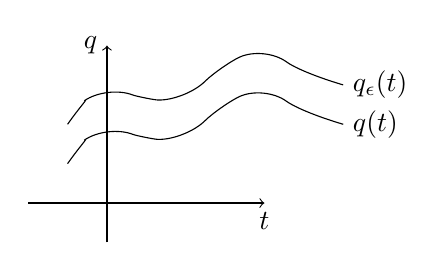
\begin{tikzpicture}[rounded corners = 10pt]
      \draw [->] (-1,0) -- (2,0) node [below] {$t$};
      \draw [->] (0,-.5) -- (0,2) node [left] {$q$};
      \draw (-.5,.5) to[bend left = 10] (0,1) to[bend right = 10] (1,.8)
        to[bend left = 10] (2,1.5) to[bend right = 10] (3,1)
        node [right] {$q(t)$};
      \draw [yshift = .5cm]
        (-.5,.5) to[bend left = 10] (0,1) to[bend right = 10]
        (1,.8)   to[bend left = 10] (2,1.5) to[bend right = 10] (3,1) node [right] {$q_\epsilon(t)$};
    \end{tikzpicture}
  \end{center}
\end{example}
\begin{example}[rotation]
  \[
    \bm q_\epsilon(t) = \bm q(t) + \epsilon \bm e_a \times q(t), \quad
    \bm f(t) = \bm e_a \times \bm q(t)
  \]
  The rotation of the world line.
  Figure: the world line rotate a angle between two time point real surface.
\end{example}
\begin{example}[time-translation]
  \[
    q_\epsilon(t) = q(t - \epsilon), \quad
    f(t) = -\dot q(t)
  \]
  \begin{center}
  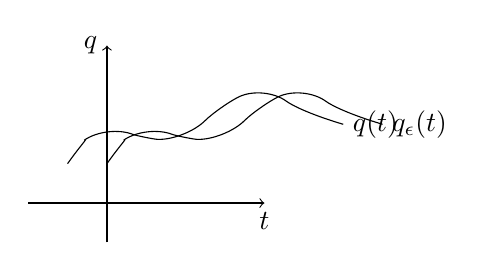
\begin{tikzpicture}[rounded corners = 10pt]
      \draw [->] (-1,0) -- (2,0) node [below] {$t$};
      \draw [->] (0,-.5) -- (0,2) node [left] {$q$};
      \draw (-.5,.5) to[bend left = 10] (0,1) to[bend right = 10] (1,.8)
        to[bend left = 10] (2,1.5) to[bend right = 10] (3,1)
        node [right] {$q(t)$};
      \draw [xshift = .5cm]
        (-.5,.5) to[bend left = 10] (0,1) to[bend right = 10]
        (1,.8)   to[bend left = 10] (2,1.5) to[bend right = 10] (3,1) node [right] {$q_\epsilon(t)$};
  \end{tikzpicture}
  \end{center}
\end{example}
For $t$-independent $\Omega_\theta$, the functional derivative
\begin{align*}
  0 & = \odv{\mathcal S[\Omega_\theta q]}\theta \bigg|_{\theta=0}
    = \frac1\epsilon (\mathcal S[\Omega_\epsilon q] - \mathcal S[q])
      \bigg|_{\epsilon \to 0}
    = \int_{t_i}^{t_f} \d t
      \ab(\pdv{\mathcal L}q \pdv{q_\theta}\theta
    + \pdv{\mathcal L}{\dot q} \pdv{\dot q_\theta}\theta) \\
    & = \int_{t_i}^{t_f} \d t
        \underbrace{\ab(\pdv{\mathcal L}q - \odv*{\pdv{\mathcal L}{\dot q}}t) f}
        _\text{E-L Equation}
      + \ab(\pdv{\mathcal L}{\dot q}f)\bigg|_{t_i}^{t_f}
\end{align*}
where we integral on shell, and
\[
  \mathcal S[q_\theta(t)] = \int_{t_i}^{t_f} \d t
  \mathcal L(q_\theta(t), \dot q_\theta(t), t)
\]
Since the E-L equation, we have
\[
  \ab(\pdv{\mathcal L}{\dot q}f)\bigg|_{t_i}^{t_f} = 0
\]
But $t_i$ and $t_f$ are arbitrary, so we can derive that
\[
  \odv*{\pdv{\mathcal L}{\dot q}f}t = 0
\]
means that it is independent from time, we get the conserved quantity.

So, in the first example $p$ is conserved; In the second one,
\[
  \mathcal S[q_\theta(t)] = \int_{t_i}^{t_f} \d t
  \mathcal L(\bm q_\theta(t), \dot{\bm q}_\theta(t), t)
\]
and
\[
  \ab(\sum_i \pdv{\mathcal L}{\dot q_i}f)\bigg|_{t_i}^{t_f} = 0
\]
so, $\bm e_a \cdot L = \bm p \cdot(\bm e_a \times \bm q(t))$
in the second example.

In the time-translation,
\[
  \mathcal S[q_\epsilon(t)] = \int_{t_i+\epsilon}^{t_f+\epsilon} \d t
  \mathcal L(q_\epsilon(t-\epsilon), \dot q_\epsilon(t-\epsilon), t)
\xlongequal{\tilde t = t - \epsilon} \int_{t_i}^{t_f} \d \tilde t
  \mathcal L(q(\tilde t), \dot q(\tilde t), \tilde + \epsilon)
\]
The derivative
\[
  0 = \odv{\mathcal S[\Omega_\theta q]}\theta \bigg|_{\theta=0}
    = \frac1\epsilon(\mathcal S[\Omega_\epsilon q] - \mathcal S[q])
    = \int_{t_i}^{t_f} \d t \pdv{\mathcal L}t \Rightarrow \pdv{\mathcal L}t = 0
\]
To interrupt it, we consider the total derivative
\[
  \odv*{\mathcal L}t = \pdv*{\mathcal L}q \dot q
+ \pdv*{\mathcal L}t\ab(\odv*{\dot q}t) + \pdv*{\mathcal L}t
\]
The second term
\[
  \pdv*{\mathcal L}t\ab(\odv*{\dot q}t)
= \odv*[fun]{\pdv{\mathcal L}q \dot q}t
- \ab(\odv*{\pdv{\mathcal L}{\dot q}}t)\dot q
\]
Substitute it and rearrange
\[
  0 = \pdv{\mathcal L}t = \odv*{\underbrace{\ab(
    \mathcal L - \pdv{\mathcal L}{\dot q} \dot q)}_\text{Hamiltonian}}t
- \underbrace{\ab(\pdv{\mathcal L}q - \odv*{\pdv{\mathcal L}q}t)}_
  \text{E-L equation} \dot q
\]
Then, we have the on-shell
\[
  \odv*{\mathcal H}t = 0
\]
i.e., the energy is conserved.

\paragraph{From (good) quantum numbers to group irrepresentation}

The statement is if
\[
  [\hat A, \hat B] = 0, \Rightarrow \exists \text{basis} \{\ket|\lambda>\}
\]
The basis vector is the eigenvector of both $\hat A$ and $\hat B$
\[
  \hat A\ket|\lambda> = \lambda_A\ket|\lambda>, \qq{and}
  \hat B\ket|\lambda> = \lambda_B\ket|\lambda>.
\]
\begin{proof}
  Consider $\hat A$ and $\hat B$ are Hermition.
  Take the ground state
  \[
    \hat A\ket|\alpha> = \alpha\ket|\alpha>
  \]
  In the case of degeneracy,
  \[
    \hat A\ket|\alpha_i> = \alpha\ket|\alpha_i>, \quad
    i = 1,\ \ldots\,,~d_\alpha
  \]
  Then, consider
  \[
    \hat A(\hat B\ket|\alpha>) = \hat B\hat A\ket|\alpha>
  = \alpha(\hat B\ket|\alpha>)
  \]
  means that
  \[
    \begin{cases*}
      \hat B\ket|\alpha> = b^{(\alpha)}\ket|\alpha>, & no-degeneracy\\
      \hat B\ket|\alpha_i> = \sum_j \ket|\alpha_j> b_{ji}^{(\alpha)}, &
      degeneracy
    \end{cases*}
  \]
  where $b_{ji}^{(\alpha)} = \braket<\alpha_j|\hat B|\alpha_i>$.
  We can always diagonalize
  \[
    b^{(\alpha_i)} = V D V^{-1}, \quad b^{(\alpha_i)} V = VD
  \]
  $D$ being a diagonal matrix $D_{ml} = \beta_l^{(\alpha)} \delta_{ml}$.
  Then,
  \[
    \sum_i b_{ji}^{(\alpha)} V_{il} = \sum_m V_{jm} D_{ml}
  = V_{jl} \beta_l^{(\alpha)}
  \]
  By take one superposition of the orginal $\alpha$
  \[
    \ket|\tilde \alpha_l> = \sum_i \ket|\alpha_i> V_{il}
  \]
  It is easy to know
  \[
    \hat B\ket|\tilde\alpha_\lambda> = \sum_i \hat B\ket|\alpha_i> V_{il}
  = \sum_{ij} \ket|\alpha_j>b_{ji}^{(\alpha)} V_{il}
  = \ket|\tilde\alpha_l> \beta_l^{(\alpha)}
  \]
  Then, the site
  \[
    \{\ket|\tilde\alpha_l>\} = \{\ket|\lambda>\}
  \]
  if there is no degeneracy, then $\ket|\tilde\alpha> = \ket|\alpha>$.
\end{proof}

\section{Symmetry group representations, degeneracies,
         inversion and time reversal}

\section{Angular momentum, Lie algebra}

\section{Gauge}


\newcommand \sectionname {Lecture \#}
\appendix
\sidefoot \thepage
\fancyhead[OL, ER]{Mingyu Xia (Westlake ID: 20251202247)}
\fancyhead[EL]{\sffamily \rightmark}
\fancyhead[OR]{\fontfamily{lmr}\selectfont<<\texttt{\href{mailto:xiamingyu@westlake.edu.cn}{xiamingyu@westlake.edu.cn}}>>}
\addcontentsline{toc}{chapter}{Problem Set}
\renewcommand *\thesection{\sectionname \arabic{section}}
\newweek
\input{homework/hw0.tex}
\newweek
\input{homework/hw1.tex}

\end{document}